



%----------------------------------------------------------------------------------------

\newpage

%\section[Interaction model][Modèle d'interaction]{Dynamical extension of the interaction model}{Extension dynamique du modèle d'interaction}
\section{Dynamical extension of the interaction model}{Extension dynamique du modèle d'interaction}



\label{sec:macrocoevol}



%----------------------------------------------------------------------------------------


Nous pouvons à présent faire la synthèse d'une part des paradigmes d'intégration d'un système de ville et du réseau de transport, effectué de manière statique pour le comportement du réseau dans le modèle d'interaction développé et exploré en section~\ref{sec:interactiongibrat}, d'autre part des indicateurs pour la compréhension d'un modèle de co-évolution pour un système de villes, expérimentés dans la section précédente~\ref{sec:macrocoevolexplo}, ainsi que de manière indicative pour comparaison des comportements obtenus pour le modèle SimpopNet. Cette synthèse consiste en une première formulation d'un \emph{modèle de co-évolution macroscopique pour les systèmes de villes}, qui est un élément clé pour apporter un éclaircissement partiel de notre problématique générale.



%%%%%%%%%%%%%%%%%
\subsection{Macroscopic Model of Co-evolution}{Modèle macroscopique de co-évolution}


%%%%%%%%%%%%%%%%%
\subsubsection{Rationale}{Hypothèses et choix de modélisation}



\bpar{
In a multi-modeling fashion, the model can take into account various processes such as between cities direct interactions, network-mediated interactions, feedback of network flows, and for the network demand-induced growth.
}{
Cette première approche se place dans une logique d'extension directe du modèle d'interactions au sein d'un système de villes présenté en chapitre~\ref{ch:evolutiveurban}, c'est à dire à une échelle macroscopique et avec une ontologie typique au systèmes de villes. Toujours dans un choix de simplicité, dont la relaxation pourra être explorée pour le cas d'application à la Chine avec l'ajout de variables économiques, nous restons ici à une description unidimensionnelle des villes par leur population. Concernant la croissance du réseau, nous proposons de se placer également à un niveau relativement agrégé et simplifié, en testant des heuristiques de croissance répondant à une demande, à différents niveaux d'abstraction. Par une forme de multi-modélisation, le modèle peut prendre en compte divers processus comme les interactions directes entre les villes, les interactions intermédiaires par le réseau, la rétroaction des flux de réseau et une croissance induite par la demande pour le réseau.
}





%%%%%%%%%%%%%%%%%
\subsubsection{General Formulation}{Formulation Générique}



%%%%%%%%%%%%%%%%%
\begin{figure}
\includegraphics[width=\linewidth]{Figures/MacroCoEvol/model}
\caption[][Schématisation du modèle]{}{\textbf{Représentation abstraite des processus du modèle.}\label{fig:macrocoevol:model}}
\end{figure}
%%%%%%%%%%%%%%%%%


Le système urbain est caractérisé par les populations $\mu_i(t)$ et le réseau $/mathbf{N}(t)$ auquel on peut associer une matrice de distance $d^N_{ij}(t)$




\paragraph{Network Growth}{Croissance du réseau}

% choice of network heuristics : less precise than meso ; more based on distance patterns.


Network growth heuristics are tested at different abstraction levels that are the time-distance matrix between cities, and physical network growth trying to satisfy greedy time-gain optimization criteria.

Given the flow $\phi$ in a link, its effective distance is updated following

For the thresholded case
\[
d(t+1) = d(t)\cdot \left( 1 + g_{max} \cdot \left[\frac{1 - \left(\frac{\phi}{\phi_0}\right)^{\gamma_s}}{1 + \left(\frac{\phi}{\phi_0}\right)^{\gamma_s}}\right]\right)
\]

where $\gamma_s$ is a hierarchy parameter, $\phi_0$ a threshold parameter and $g_{max}$ the maximal growth rate easily adjustable to realistic values by computing $(1+g_{max})^{t_f}$






\subsubsection{Implementation}{Implémentation}



\bpar{
}{
Le couplage du modèle d'interaction à la prise en compte plus fine des processus de réseau rend plus difficile l'intégration complète dans un plugin OpenMole comme c'était le cas pour le modèle étudié en~\ref{sec:interactiongibrat}. L'utilisation d'un workflow comme médiateur pour le couplage est une solution intéressante mais réaliste uniquement dans le cas d'un couplage faible. L'un des défis que devra relever la bibliothèque de méta-modélisation en cours de développement autour d'OpenMole, serait la possibilité de coupler fortement (par exemple au sens de dynamiquement dans l'évolution de la simulation) des composantes hétérogènes de manière transparente. Nous optons pour ce modèle pour une implémentation complète en NetLogo pour une simplicité de couplage des composantes. Une attention particulière est portée à la dualité de la représentation du réseau, à la fois sous forme de matrice de distance et sous forme physique.
}






%%%%%%%%%%%%%%%%%
\subsection{Application to Synthetic Data}{Application à des Données Synthétiques}


\bpar{
The model is first tested and explored on synthetic city systems, generated following a simple heuristic to follow the rank-size law and Central Place Theory.
%The systematic exploration through intensive computation unveils different interaction regimes across the parameter space. In some, the introduction of the network can drastically change the fate of some cities, whereas the top-distribution hierarchy is reinforced, what is consistent with empirical observations in the literature. Some regimes suggest circular causalities between network and city growth, corresponding to the co-evolution.
}{
Le modèle est d'abord testé et exploré sur des systèmes de villes synthétiques, afin de comprendre certaines de ses propriétés intrinsèques. Dans ce cas, nous considérons le modèle avec réseau abstrait, c'est à dire sans explicitation spatiale du réseau et avec les règles d'évolution agissant directement sur $d_{ij}$ selon les spécifications données précédemment.
}


\paragraph{Synthetic data}{Données Synthétiques}

Un système de villes synthétiques est généré de la façon la plus simple possible, en suivant l'heuristique utilisée dans la section précédente : (i) des villes en nombre $N_S$ sont placées aléatoirement dans le plan euclidien\footnote{nous relâchons la possible contrainte de positionnement selon des logiques de places centrales} ; (ii) les populations sont attribuées aux villes selon une hiérarchie $\alpha_S$, de telle façon que la plus grande ville ait une population $P_{max}$, c'est-à-dire suivant $P_i = P{max} \cdot i^{-\alpha_S}$. Pour simplifier, le nombre de ville est fixé à $N_S = 30$ et la population maximale à $P_{max} = 100000$.


\paragraph{Results}{Résultats}


Nous explorons une grille de l'espace des paramètres $(\alpha_S,\phi_0,\gamma_s,w_G,d_G,\gamma_G)$. Nous utilisons les indicateurs introduits en~\ref{sec:macrocoevolexplo} pour quantifier le comportement du modèle dans l'espace des paramètres. En Fig.~\ref{fig:macrocoevol:behavior}, nous montrons l'évolution d'indicateurs dans le temps ainsi que des mesures agrégées, pour une grande partie de l'espace des paramètres couvert. L'évolution de la centralité de proximité moyenne dans le temps, visualisée pour $w_G = 0.001$, et à $(d_G,\gamma_G,\phi_0)$ variables, témoigne d'une transition en fonction du niveau de hiérarchie : lorsque celui-ci décroit, on observe l'émergence de trajectoires où la centralité moyenne croît dans le temps, ce qui correspond à des situations où l'ensemble des villes bénéficie d'accroissements d'accessibilité. En terme d'entropie des populations, l'ensemble des paramètre donne une entropie décroissante, c'est à dire des convergences des trajectoires dans le temps. Lorsqu'on s'intéresse à la complexité des trajectoires d'accessibilité, on note pour des valeurs de $\phi_0 > 1.5$ un maximum de la complexité en fonction de la distance d'interaction $d_G$, consistant lorsque $w_G$ et $\gamma_G$ varient. Cette échelle intermédiaire peut être interprétée comme produisant des sous-systèmes régionaux, assez grands pour développer chacun un certain niveau de complexité, et assez isolés pour ne pas uniformiser les trajectoires sur l'ensemble de l'espace. On reconstruit ainsi une non-stationnarité spatiale, typiquement observée en~\ref{sec:staticcorrelations}, et rejoignons le concepts de niche écologique localisée dans l'espace (voir~\ref{sec:theory}). Enfin, le comportement des correlations de rang pour l'accessibilité révèle que la distance d'interaction augmente systématiquement le nombre d'inversions de hiérarchie, ce qui correspond en un sens à une augmentation de la complexité globale du système. Le paramètre de hiérarchie diminue quant à lui cette corrélation, ce qui veut dire qu'une évolution plus hiérarchique affectera un plus grand nombre de villes dans l'aspect qualitatif de leur trajectoires.



%%%%%%%%%%%%%
\begin{figure}
%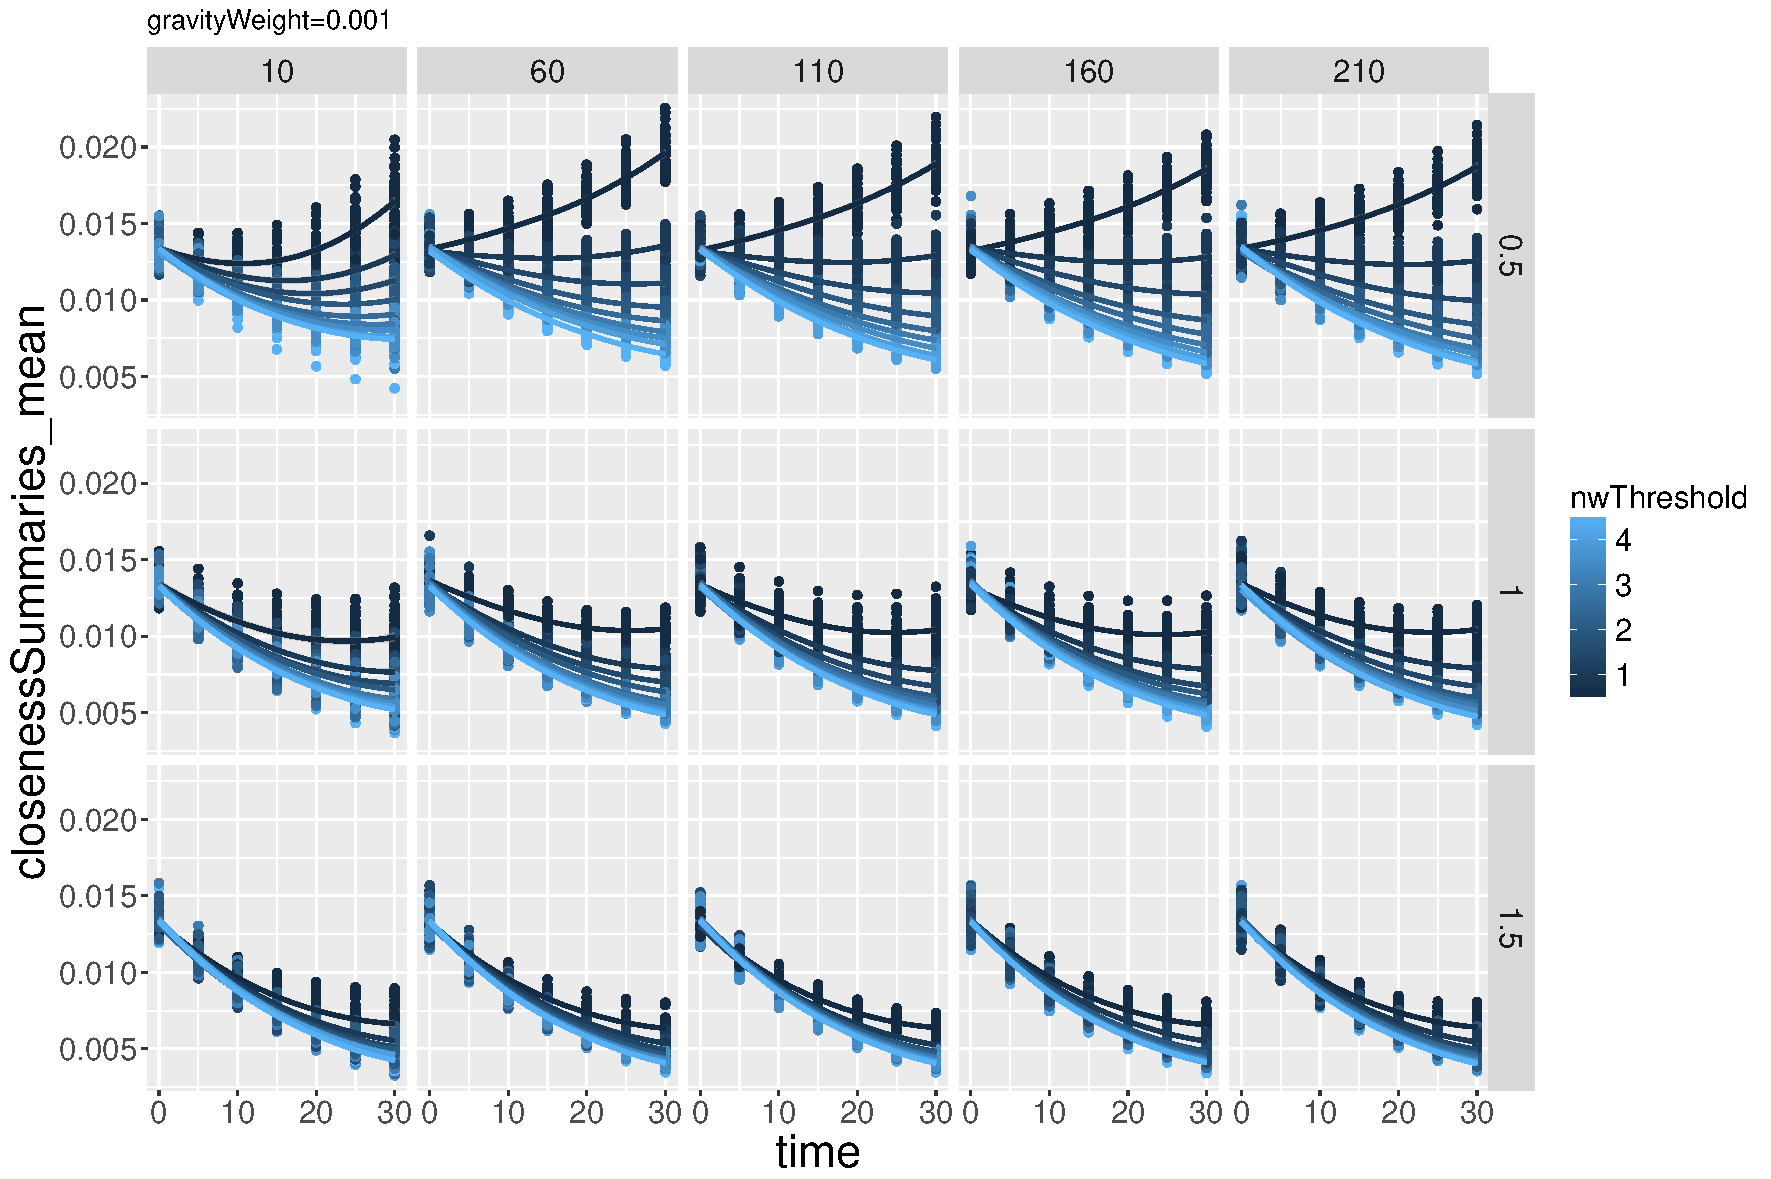
\includegraphics[width=0.48\linewidth]{Figures/MacroCoEvol/closenessSummaries_mean_gravityWeight0_001}
%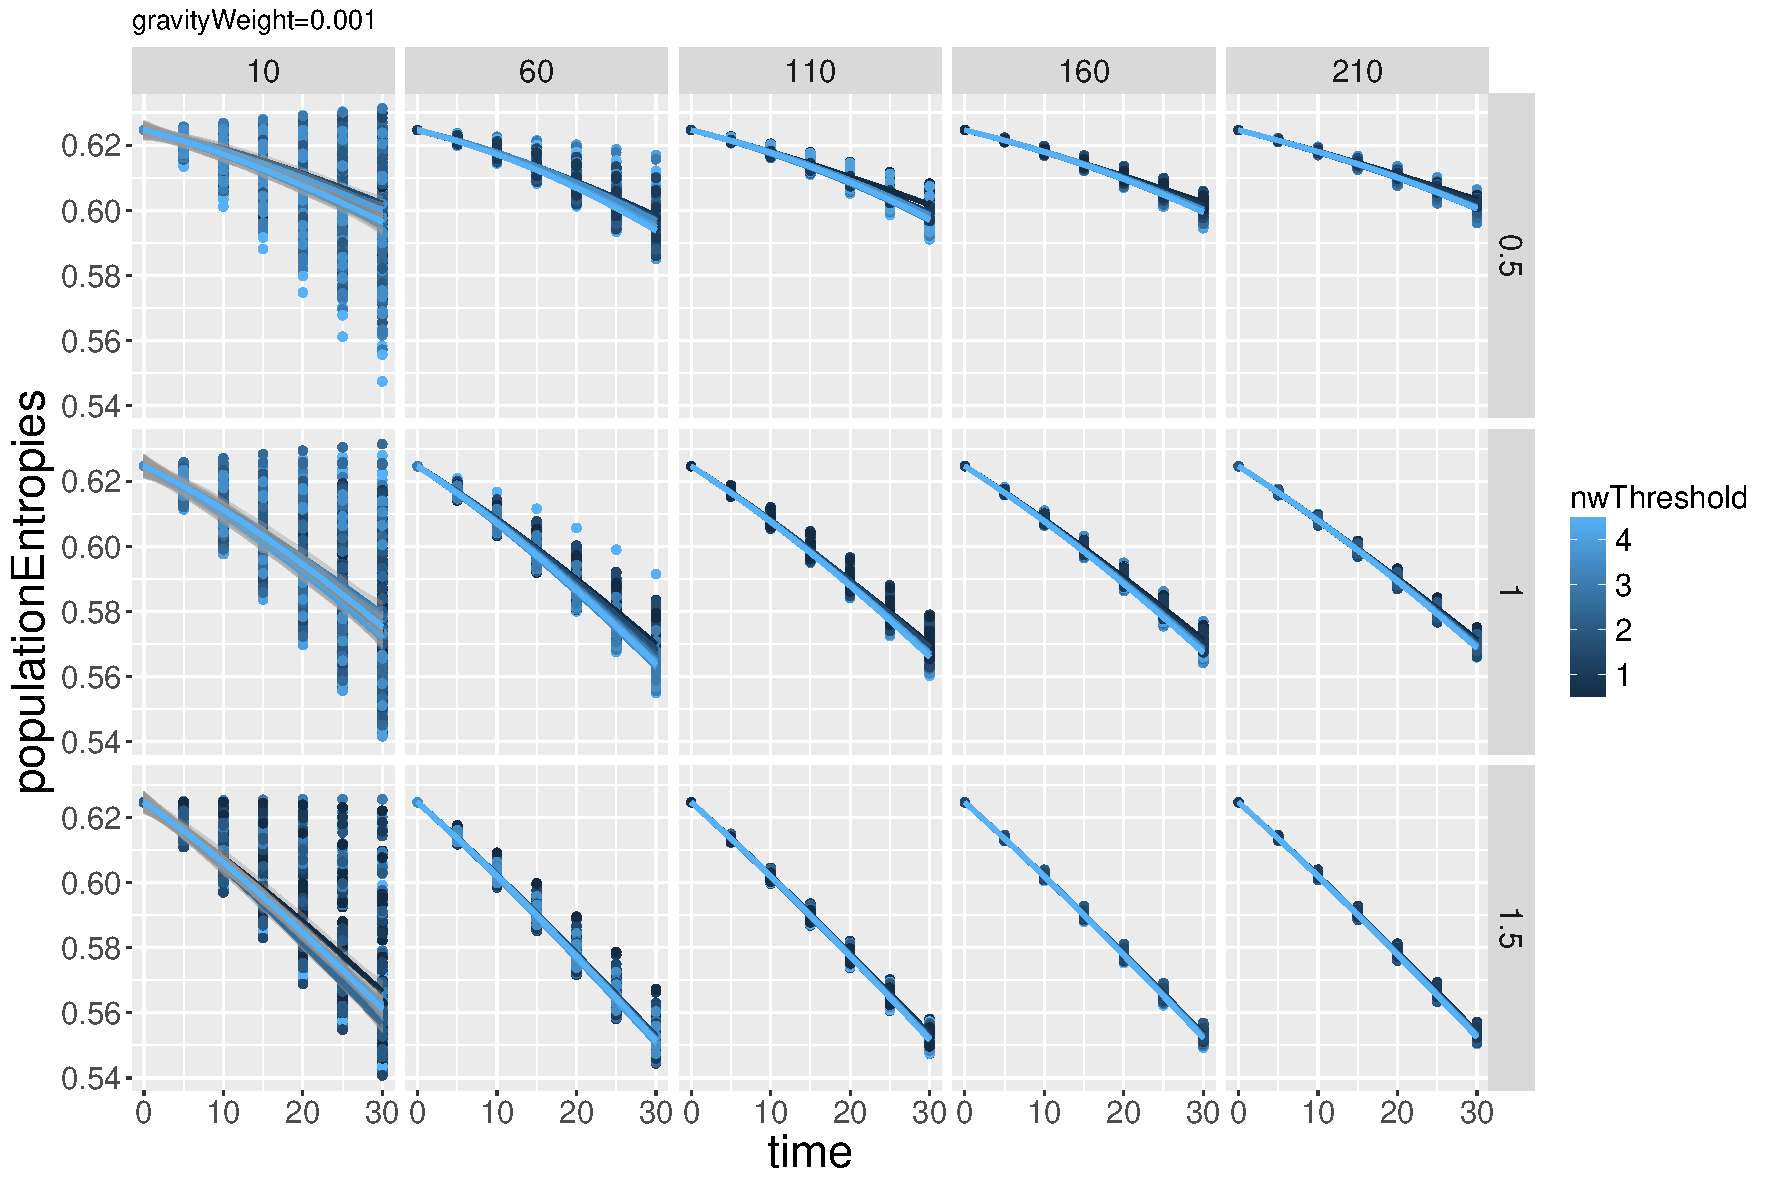
\includegraphics[width=0.48\linewidth]{Figures/MacroCoEvol/populationEntropies_gravityWeight0_001}\\
%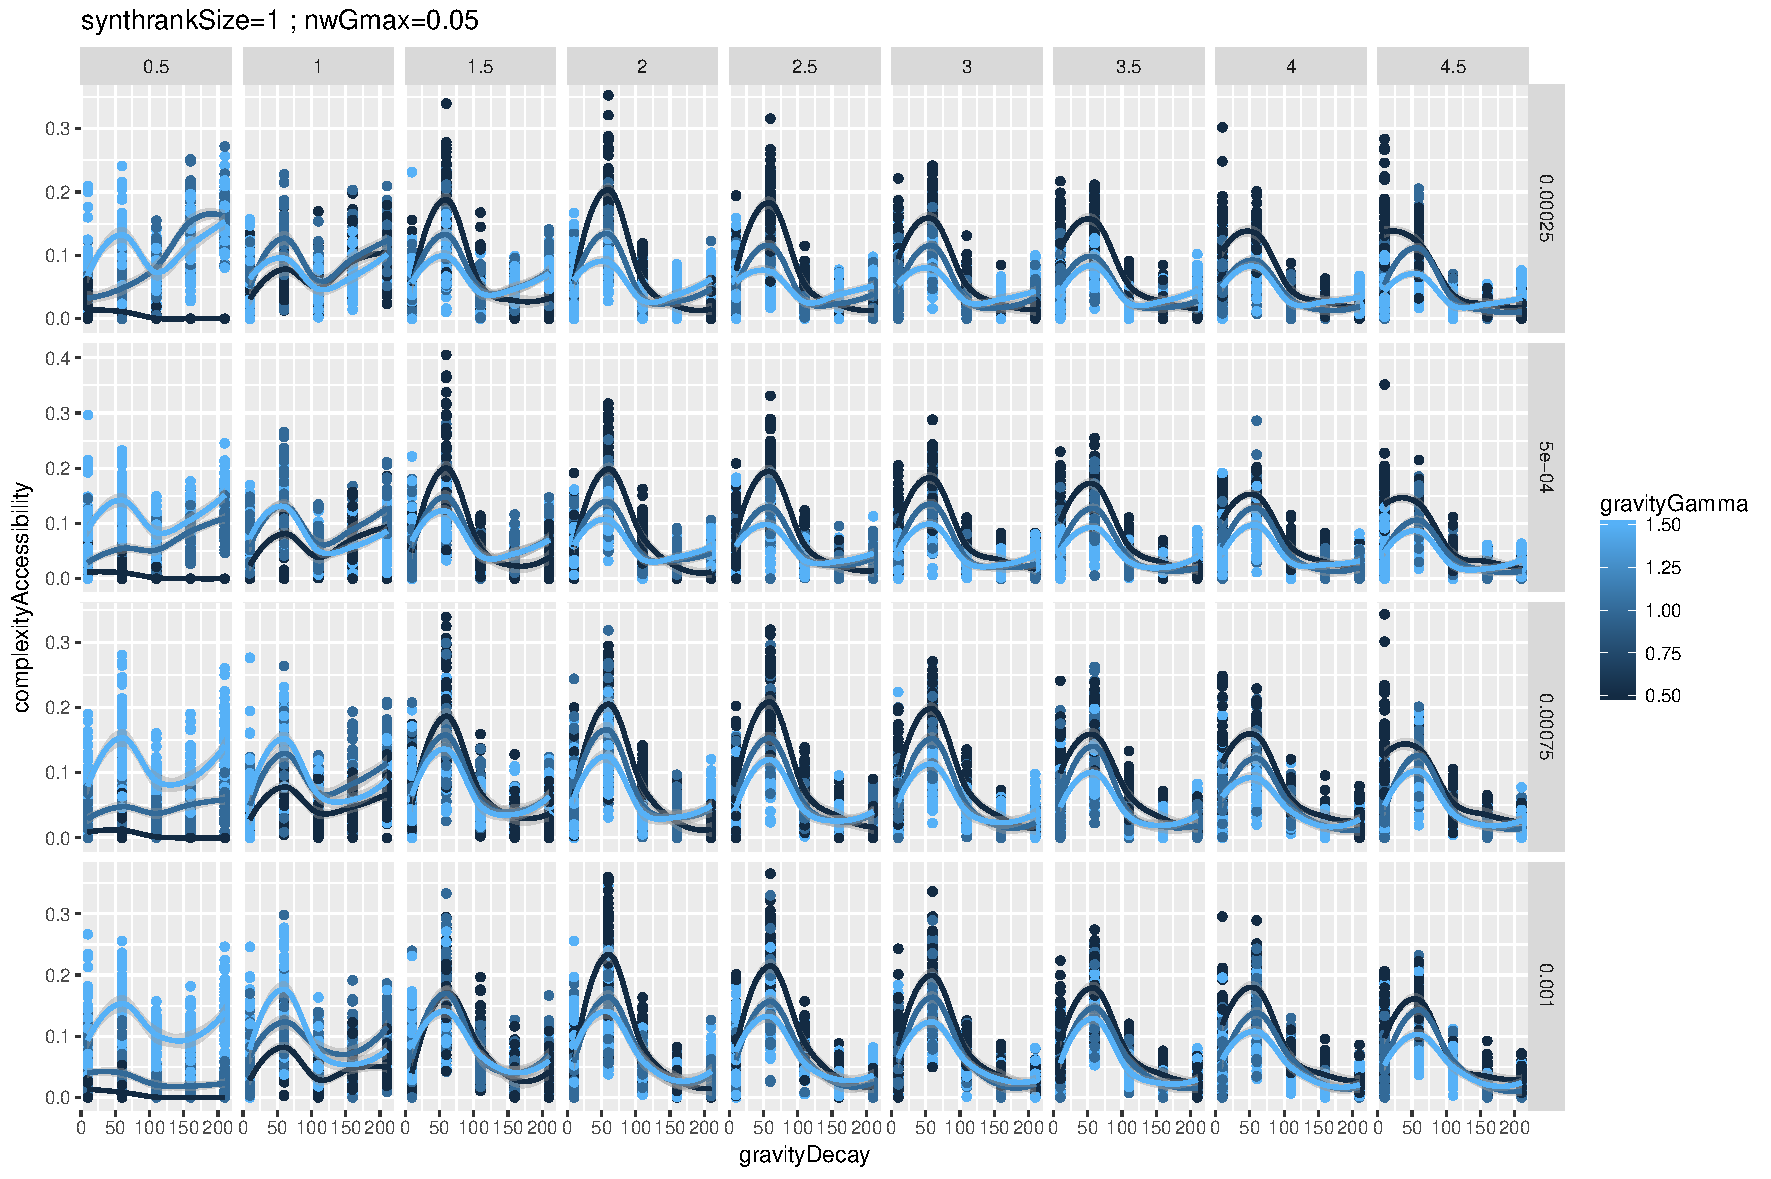
\includegraphics[width=0.48\linewidth]{Figures/MacroCoEvol/complexityAccessibility_synthrankSize1_nwGmax0_05}
%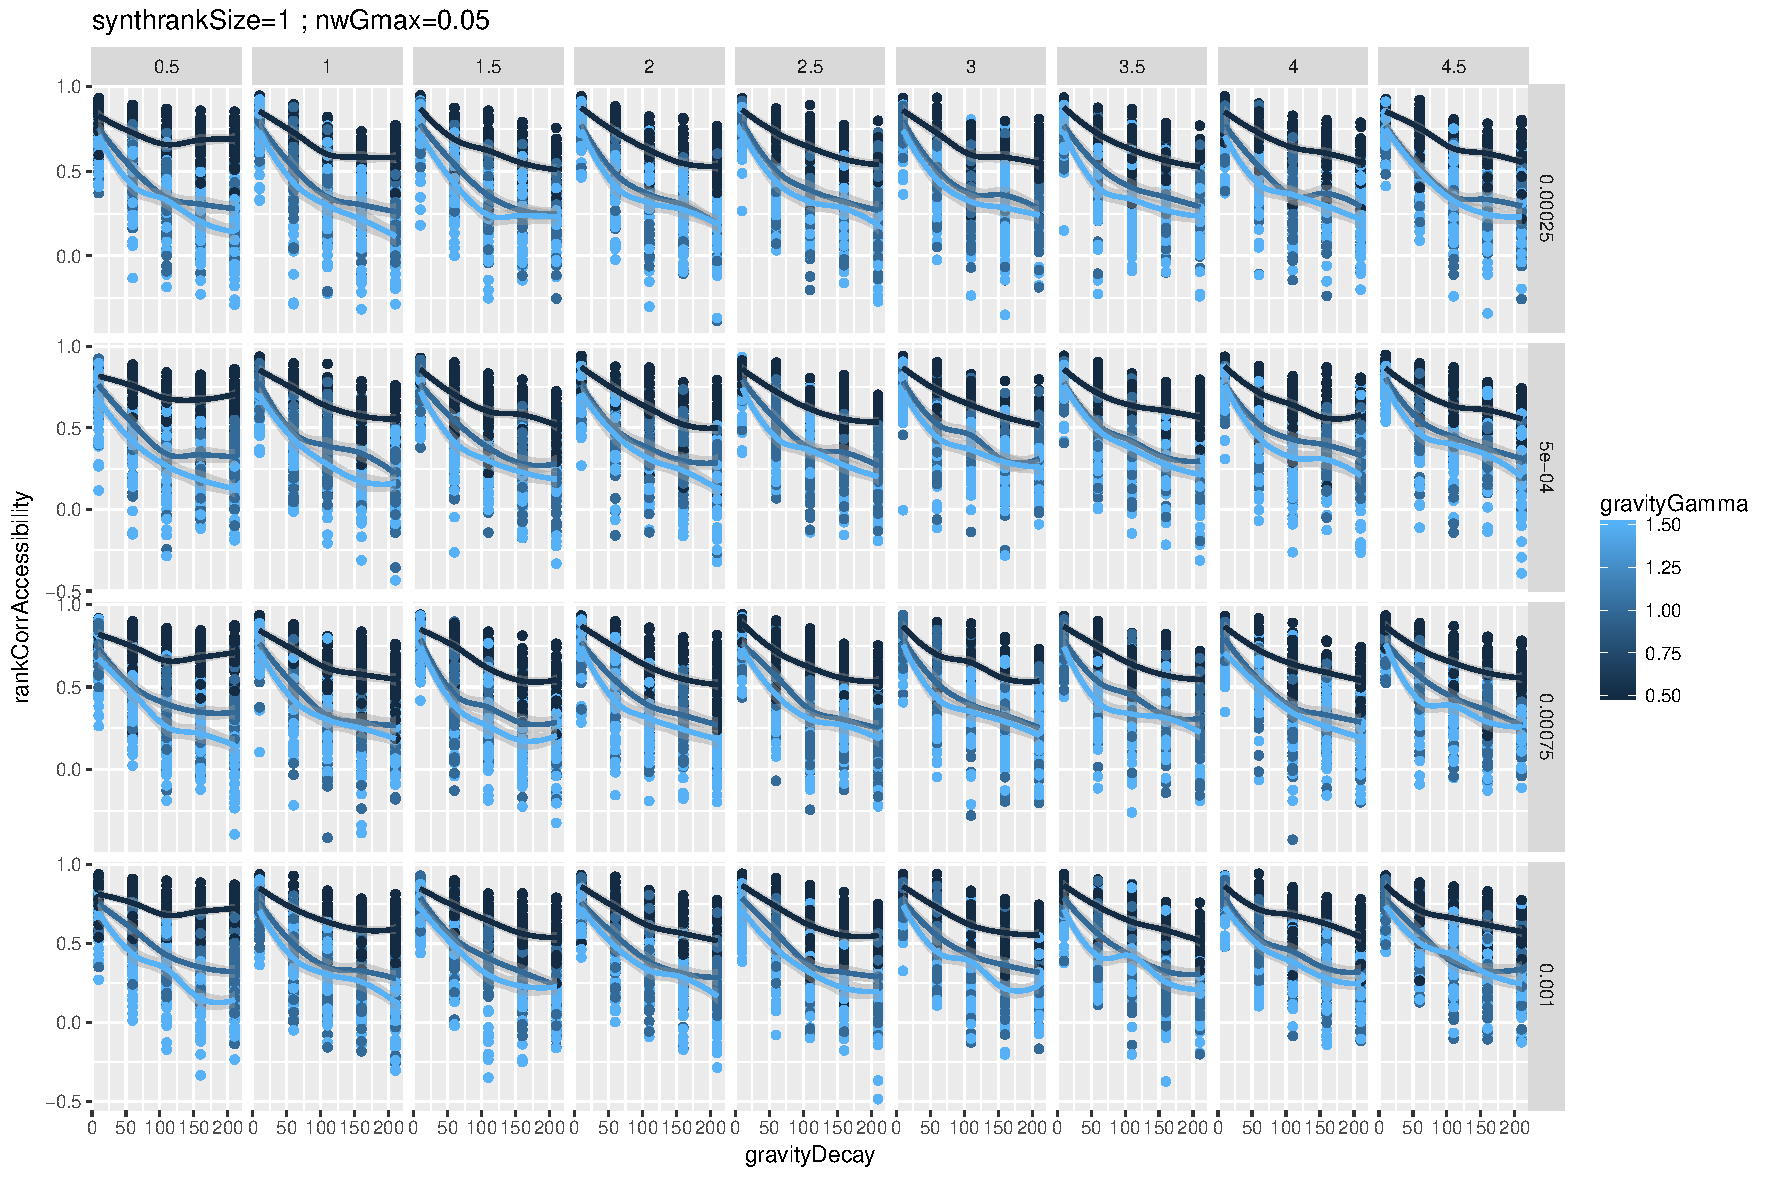
\includegraphics[width=0.48\linewidth]{Figures/MacroCoEvol/rankCorrAccessibility_synthrankSize1_nwGmax0_05}
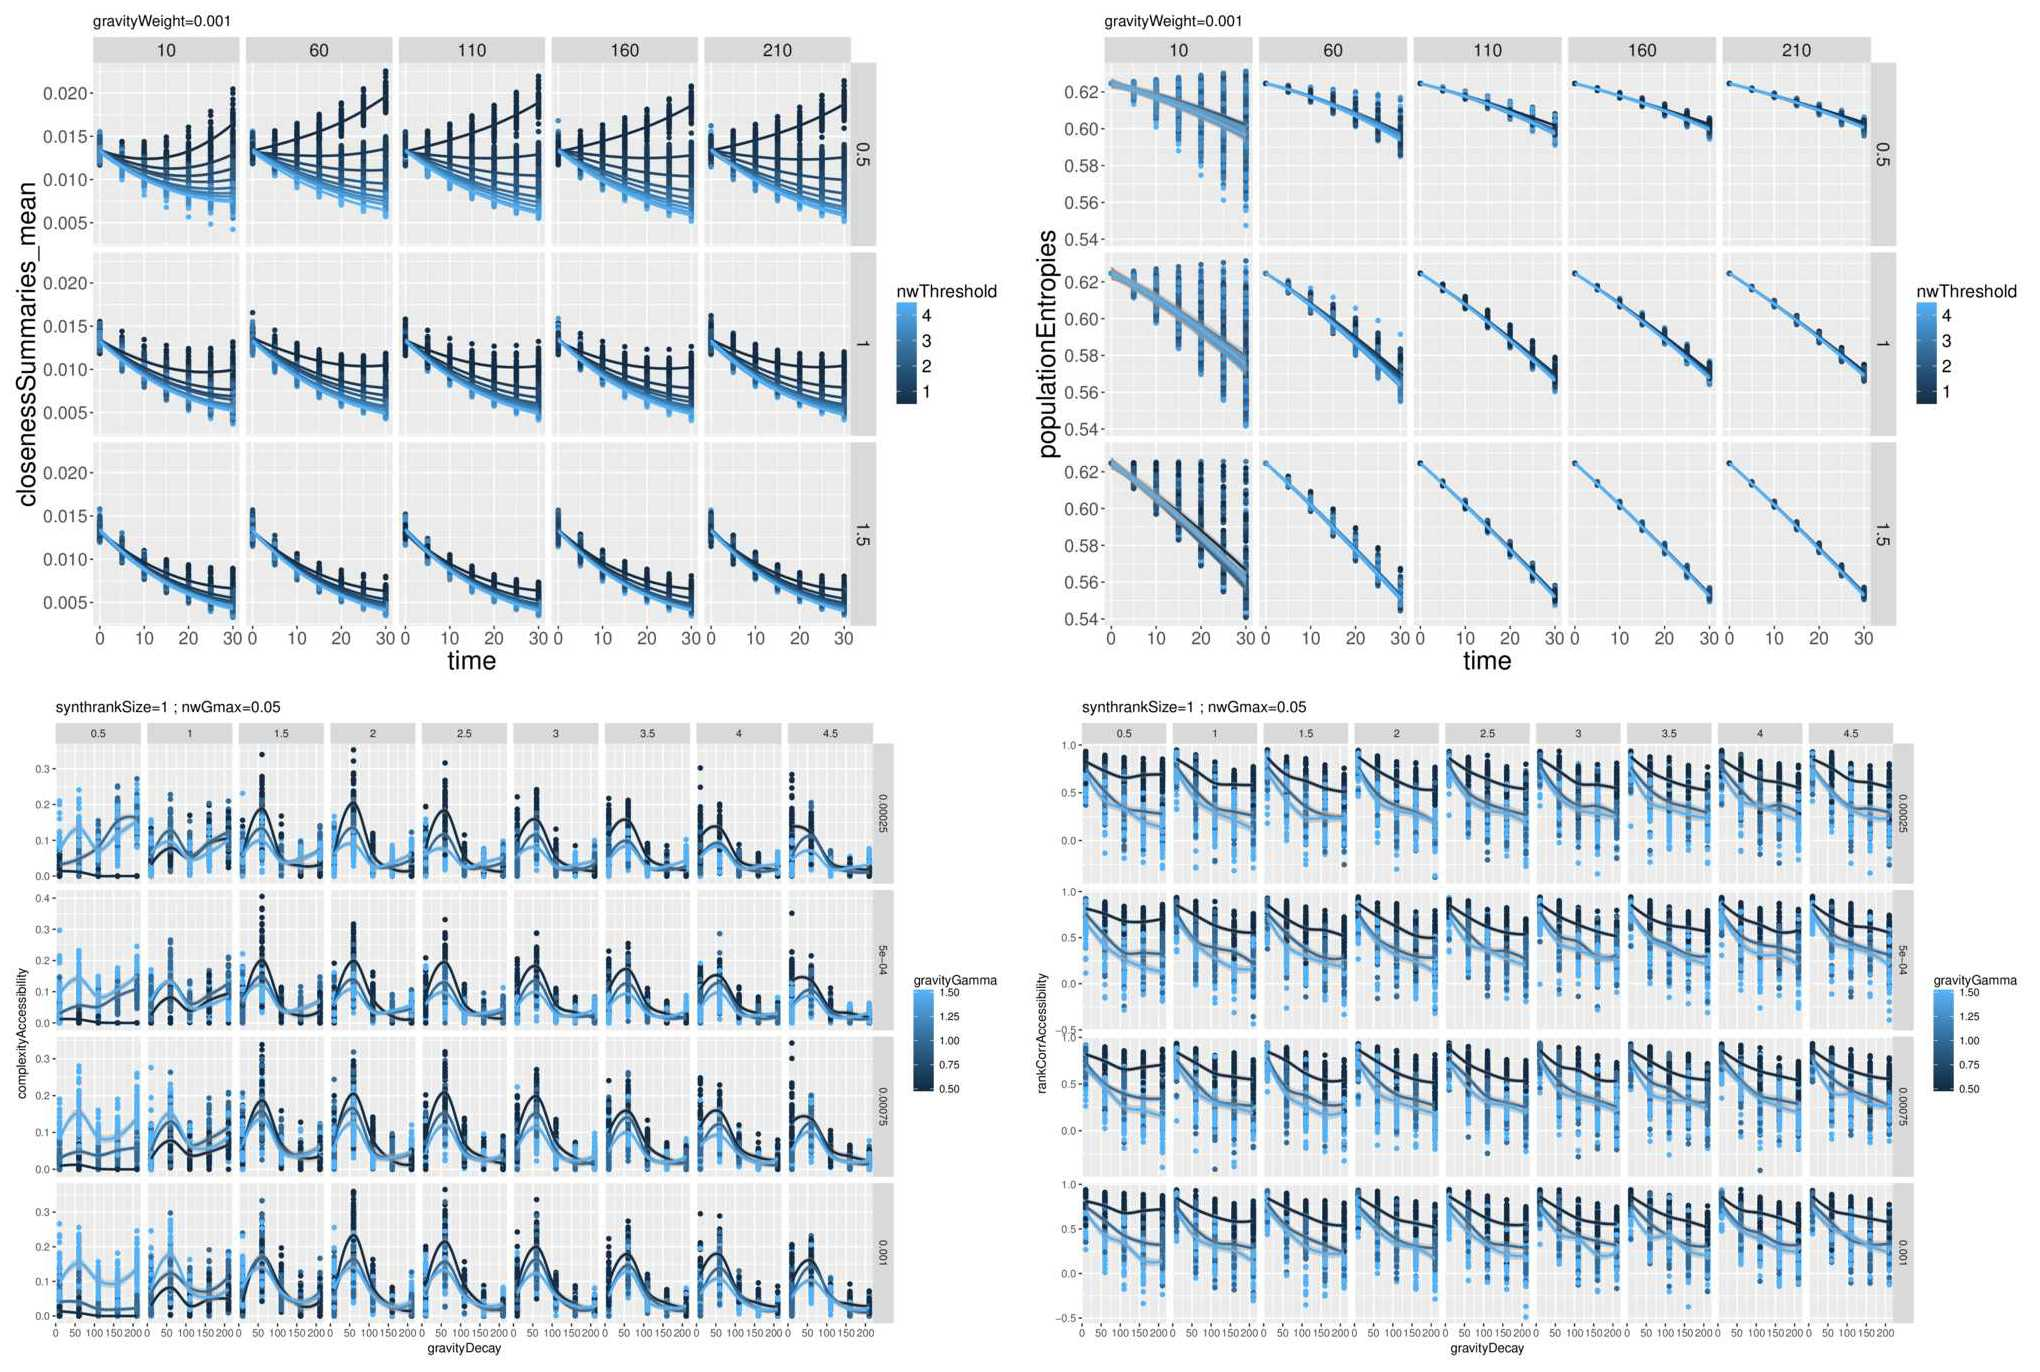
\includegraphics[width=\linewidth]{Figures/Final/6-2-2-fig-macrocoevol-behavior.jpg}
\caption[Behavior of the co-evolution model][Comportement du modèle de co-evolution]{\textbf{Behavior of the co-evolution model.}\label{fig:macrocoevol:behavior}}{\textbf{Comportement du modèle de co-evolution avec réseau abstrait sur un système de villes synthétique.} \textit{(Haut Gauche)} Moyenne des centralités de proximité, en fonction du temps, pour $d_G$ (colonnes), $\gamma_G$ (lignes) et $\phi_0$(couleur) variables, à $w_G = 0.001$ fixé ; \textit{(Haut Droite)} Entropie de populations, en fonction du temps, pour $d_G$ (colonnes), $\gamma_G$ (lignes) et $\phi_0$(couleur) variables, à $w_G = 0.001$ fixé ; \textit{(Bas Gauche)} Complexité des accessibilités, en fonction de $d_G$, pour $\phi_0$ (colonnes), $w_G$ (lignes) et $\gamma_G$ variables, avec $\alpha_S = 1$ et $g_{max} = 0.05$ ; \textit{(Bas Droite)} Corrélations de rang des accessibilités, pour les mêmes paramètres. Se référer au texte pour l'interprétation.\label{fig:macrocoevol:behavior}}
\end{figure}
%%%%%%%%%%%%%




%%%%%%%%%%%%%
\begin{figure}
	%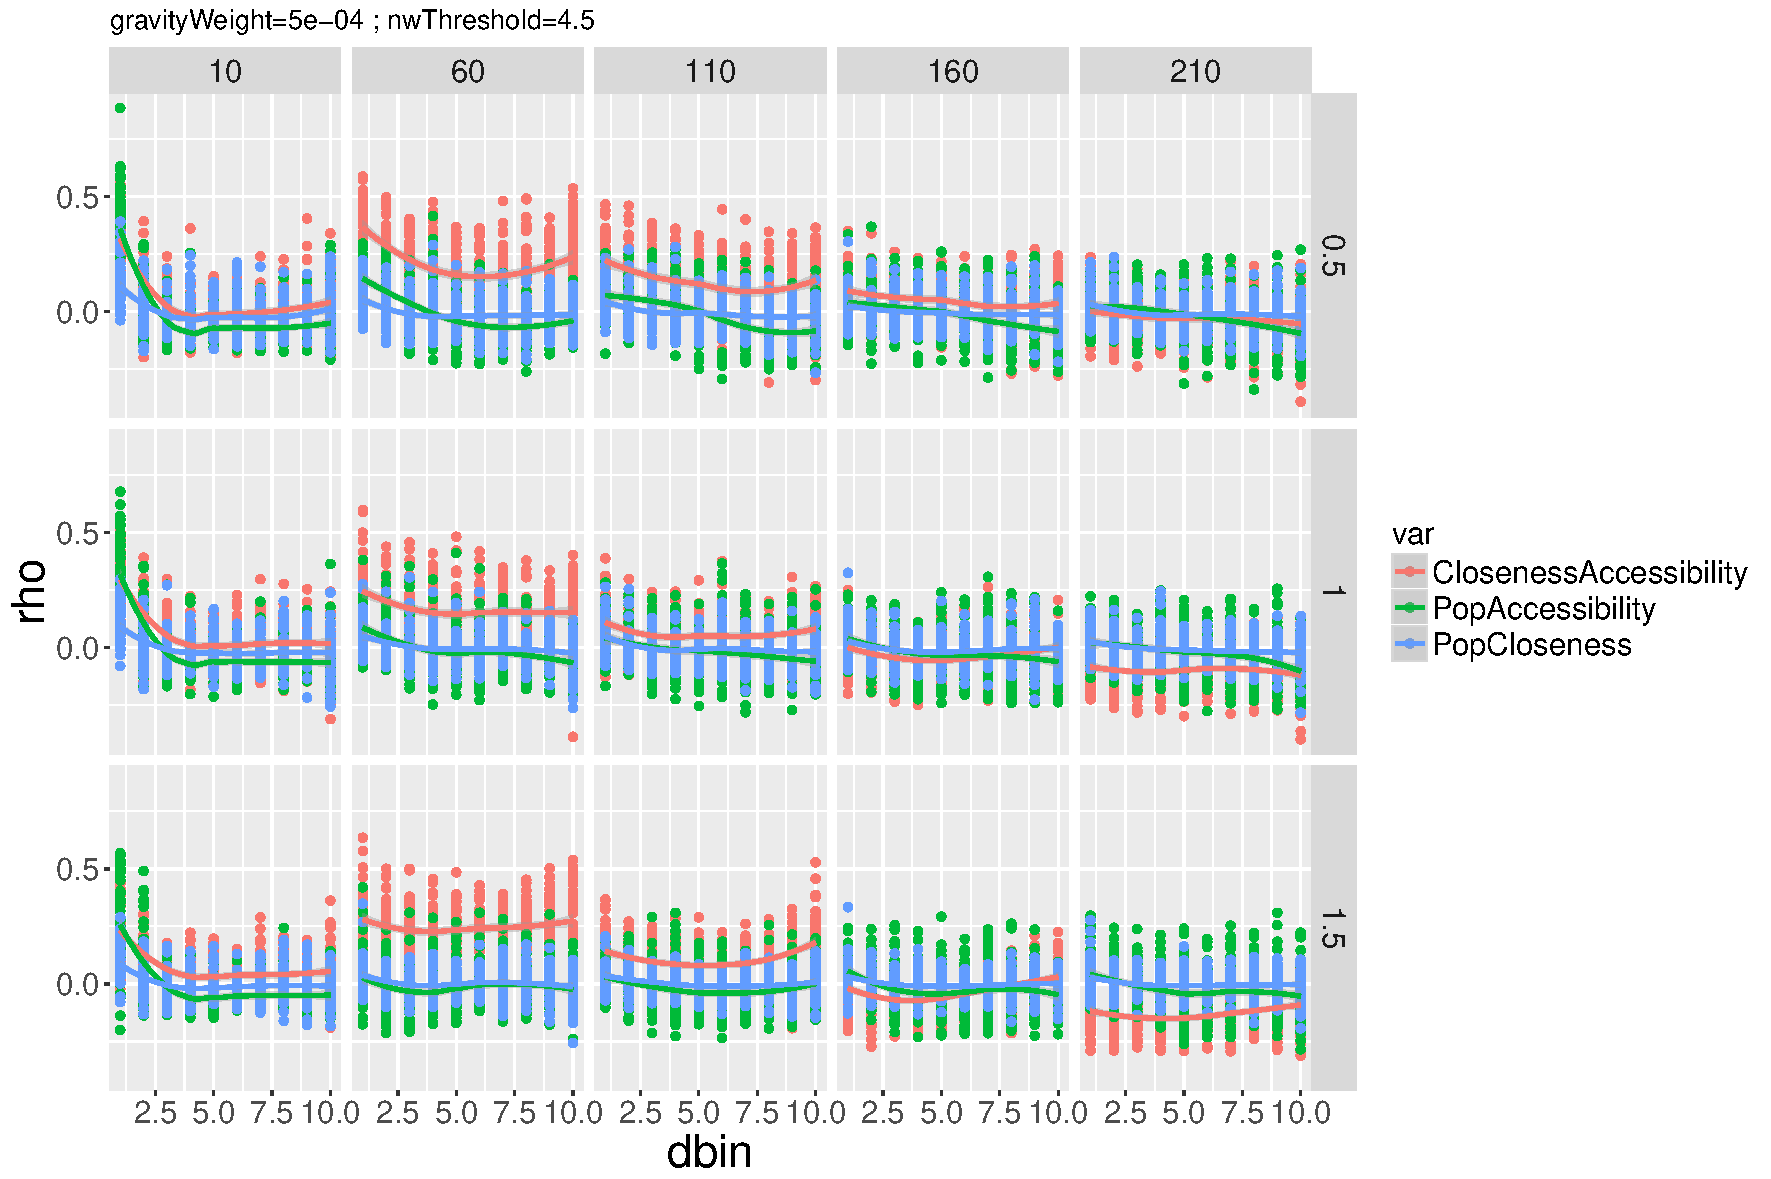
\includegraphics[width=0.9\linewidth]{Figures/MacroCoEvol/distcorrs_gravityWeight5e-04_nwThreshold4_5}\\
	%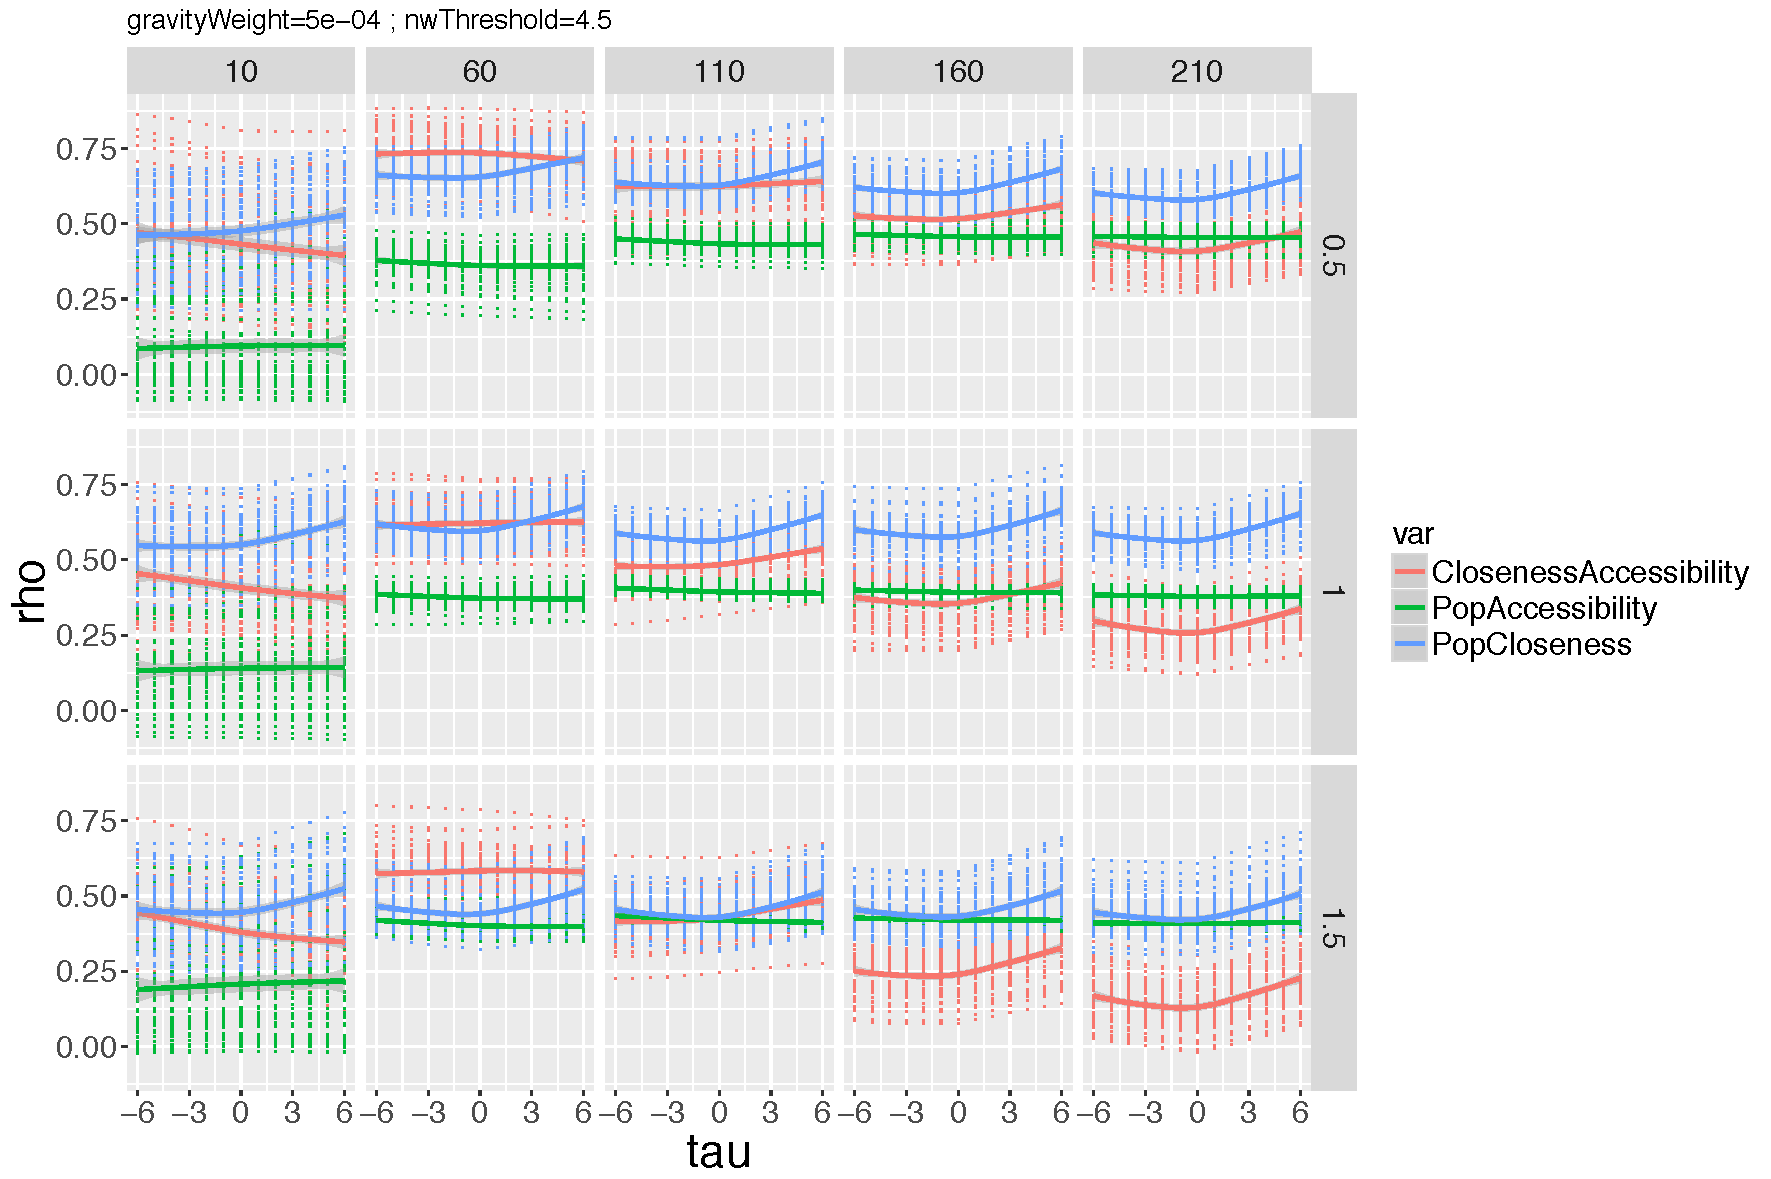
\includegraphics[width=0.9\linewidth]{Figures/MacroCoEvol/laggedcorrs_gravityWeight5e-04_nwThreshold4_5}
	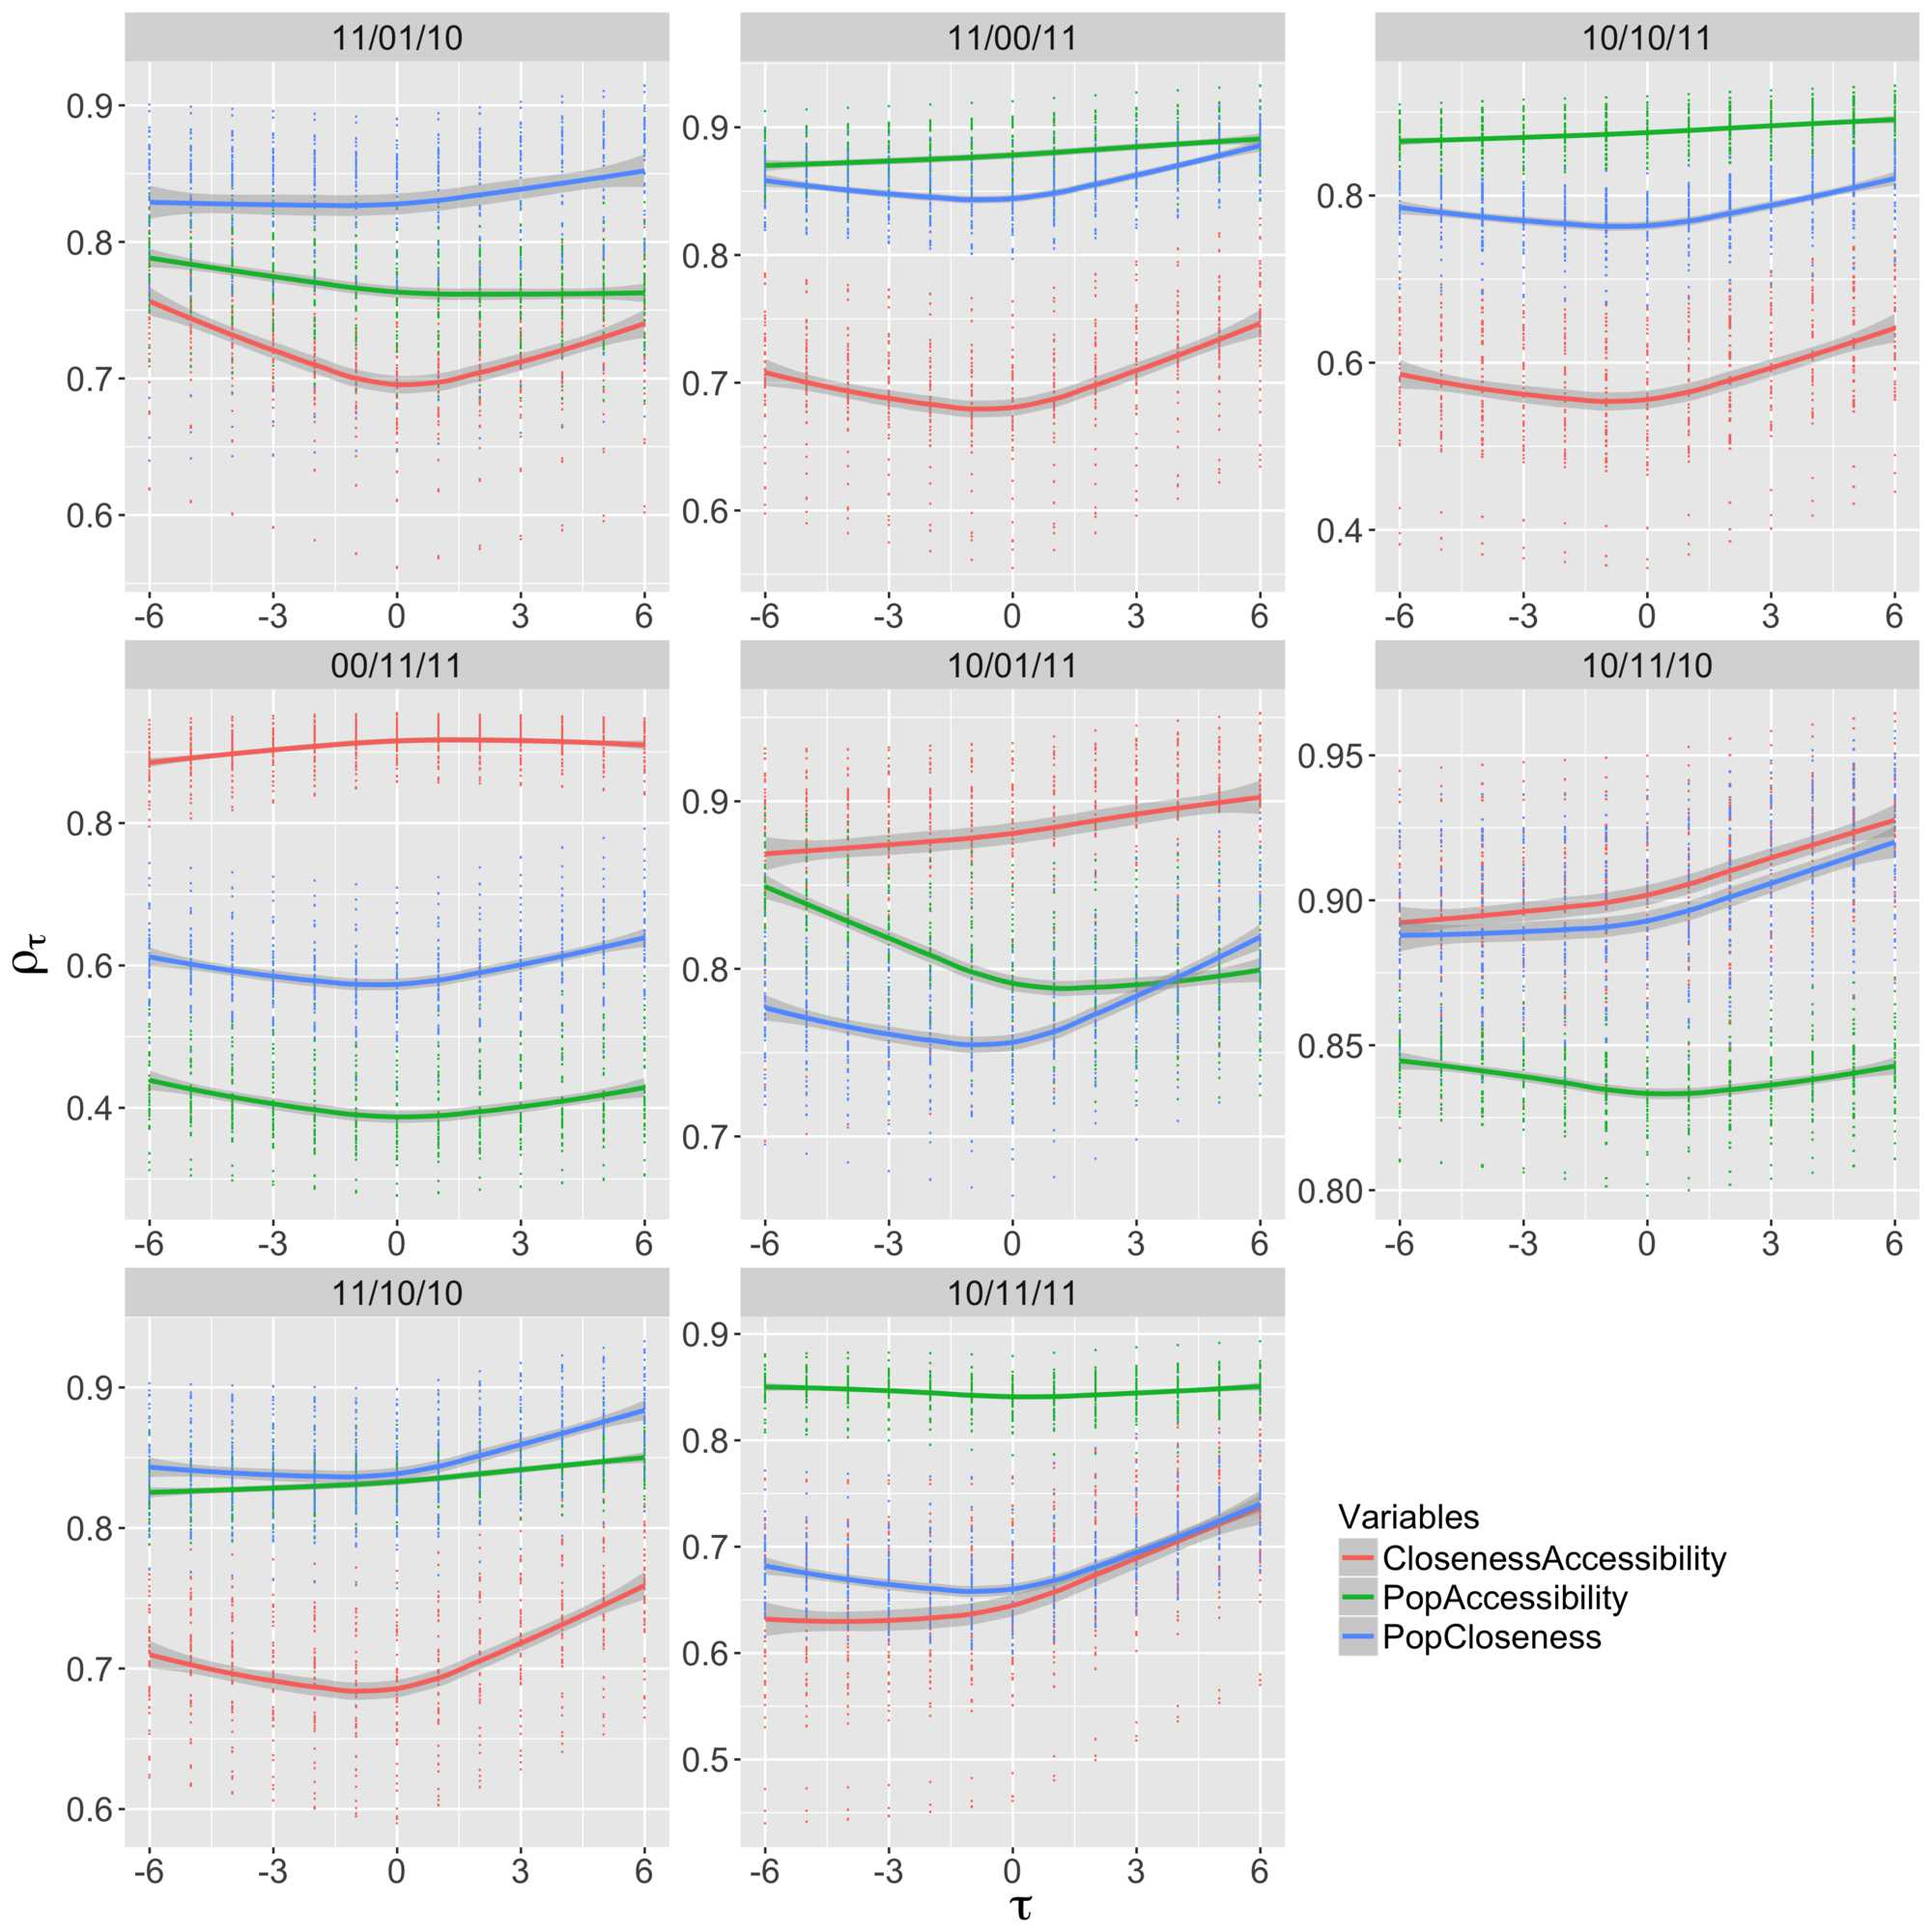
\includegraphics[width=\linewidth]{Figures/Final/6-2-2-fig-macrocoevol-correlations.jpg}
\caption[Correlations in the abstract model][Correlations dans le modèle abstrait]{}{\textbf{Motifs de correlation dans le modèle abstrait.} \textit{(Haut)} Correlation $\rho_d$ entre couples de variables (donné par la couleur), en fonction de la distance $d$ (discrétisée en déciles), pour $d_G$ variable (colonnes) et $\gamma_G$ variable (lignes), à $w_G = 5e-4$ et $\phi_0 = 4.5$ ; \textit{(Bas)} Correlations retardées $\rho_{\tau}$ en fonction du retard $\tau$, de manière similaire pour $d_G$ variable (colonnes) et $\gamma_G$ variable (lignes), à $w_G = 5e-4$ et $\phi_0 = 4.5$. \label{fig:macrocoevol:correlations}}
\end{figure}
%%%%%%%%%%%%%


Tournons nous à present vers les motifs de corrélation produits par le modèle, illustrés en Fig.~\ref{fig:macrocoevol:correlations}. En fonction de la distance, les profils de $\rho_d$ pour les trois couples de variables montrent que des valeurs moyennes et grandes de la distance d'interaction ($d_G > 50$) décorrèlent totalement population avec centralité et accessibilité. Pour des petits $d_G$, un profil décroissant puis nul confirme l'existence d'effets locaux forts, où des villes très proches s'influenceront fortement. Le comportement de la correlation entre accessibilité et centralité est plus difficile à interpréter, et peut être dû aux phénomènes d'auto-correlation\footnote{qui ne sont pas calculables, car il s'agirait de décomposer $\rho\left[\sum_{i\neq j} \frac{1}{d_{ij}}; \sum_{i\neq j} P_j \exp{\left(-d_{ij}/d_G\right)}\right]$. Il est possible par exemple d'approximer $\rho\left[X+Y;Z\right]$ sous la condition que $\varepsilon = \sigma_Y / \sigma_X \ll 1$ au premier ordre par $\rho\left[ X+Y;Z \right] \simeq \rho\left[ X;Z \right]\left(1+\frac{1}{2}\rho\left[X;Y\right]\varepsilon - \frac{\varepsilon^2}{2})\right) + \varepsilon \rho\left[Y;Z\right]$, mais cette hypothèse est trop restrictive pour être valable sur l'ensemble de la somme.}. Son niveau ne dépend pas de la distance mais de $d_G$, et est décroissant pour finir à une corrélation négative. Enfin, concernant les corrélations retardées, on observe systématiquement une déviation positive de la corrélation entre population et accessibilité pour les retards positifs, en croissance jusqu'au retard maximal, ce qui pourrait être un marqueur du renforcement des dynamiques de population par la centralité, fait stylisé exhibé pour le système de ville Français par~\cite{bretagnolle:tel-00459720}. La correlation entre population et accessibilité est constante, probablement par l'auto-corrélation, et n'entre pas en jeu dans la définition des régimes. Pour des valeurs intermédiaires de $d_G$ et les fortes valeurs de $\gamma_G$, on observe également une très légère déviation pour les retards négatifs : pour ces régimes, on a causalité circulaire et le modèle capture une co-évolution dans ce sens. L'accessibilité quant à elle cause fortement la centralité pour $d_G = 10$, puis la tendance s'inverse pour les grands $d_G$. Pour $d_G = 10$, cela va dans le sens du lien entre population et centralité, et il n'y a dans ce cas pas co-évolution mais adaptation des populations au réseau. Pour les régimes intermédiaire, on a circularité directement entre population et centralité, tandis que pour $d_G > 110$ il y a ``circularité indirecte'', puisque accessibilité cause centralité qui cause population (qui entre en jeu dans la centralité). Ainsi, le modèle capture au moins trois régimes de co-évolution distincts, en fonction de la distance d'interaction et du niveau de hiérarchie\footnote{Une analyse plus systématique par apprentissage non-supervisé comme en~\ref{sec:causalityregimes} et en~\ref{sec:mesocoevolmodel} est laissée pour de futures développements.}.







\paragraph{Synthesis}{Synthèse}

Les faits stylisés marquants qui ressortent de l'exploration du modèle synthétique sont les suivants :

\begin{enumerate}
	\item On démontre l'existence d'une échelle spatiale intermédiaire permettant l'évolution de niches relativement indépendantes, correspondant à un niveau de complexité des trajectoires maximal.
	\item Les corrélations retardées mettent en évidence au moins trois régimes différents d'interaction, que l'on interprète comme un régime d'adaptation, un régime de co-évolution direct et un régime de co-évolution indirecte.
\end{enumerate}





%%%%%%%%%%%%%%%%%
%\subsection[Application][Application]{Applications to Case Studies}{Applications au Système de Villes Français}
\subsection{Applications to French City System}{Applications au Système de Villes Français}



\bpar{
The model is applied to the French Urban System on long time dynamical data : Pumain-INED database for populations spanning between 1831 and 1999, with the evolving railway network from 1840 to 2000.
}{
Le modèle est ensuite appliqué au système de villes français sur des données dynamiques sur le temps long : la base Pumain-INED pour les populations, couvrant de 1831 à 1999, avec le réseau ferré dynamique de 1840 à 2000. Cette application vise d'une part à tester la capacité du modèle à reproduire une dynamique de co-évolution réelle, et d'autre part à extraire une information thématique sur les processus impliqué via les valeurs calibrées des paramètres.
}



\subsubsection{Network Data}{Données de Réseau}

Nous travaillons sur les données de réseau ferré construites par~\cite{thevenin2013mapping}. Le réseau ferré français est particulièrement intéressant en conjonction avec les données de population déjà présentées, puisque la période couverte est relativement similaire, et que ce moyen de transport a à toute période concrétisé l'implication d'acteurs publiques et privés importants, tout en exhibant différents régimes selon les époques, d'une gestion plutôt décentralisée à une centralisation très forte plus récemment, et différentes concrétisations technologiques avec par exemple l'émergence récente de la grande vitesse. Pour chaque date de la base de donnée de population, nous extrayons le graphe abstrait simplifié où toutes les gares et intersections de degré supérieur à deux sont reliés par les liens abstrait avec attributs de vitesse et distance traduisant la valeur réelle, à une granularité de 1km. Cela permet également de construire les matrice de distance-temps entre les villes considérées dans le modèle.





%%%%%%%%%%%%%%%%%%%%
%% On hold

%\subsubsection{Stylized facts}{Faits stylisés}
% correlation patterns in real data.





%%%%%%%%%%%%%
\begin{figure}
	%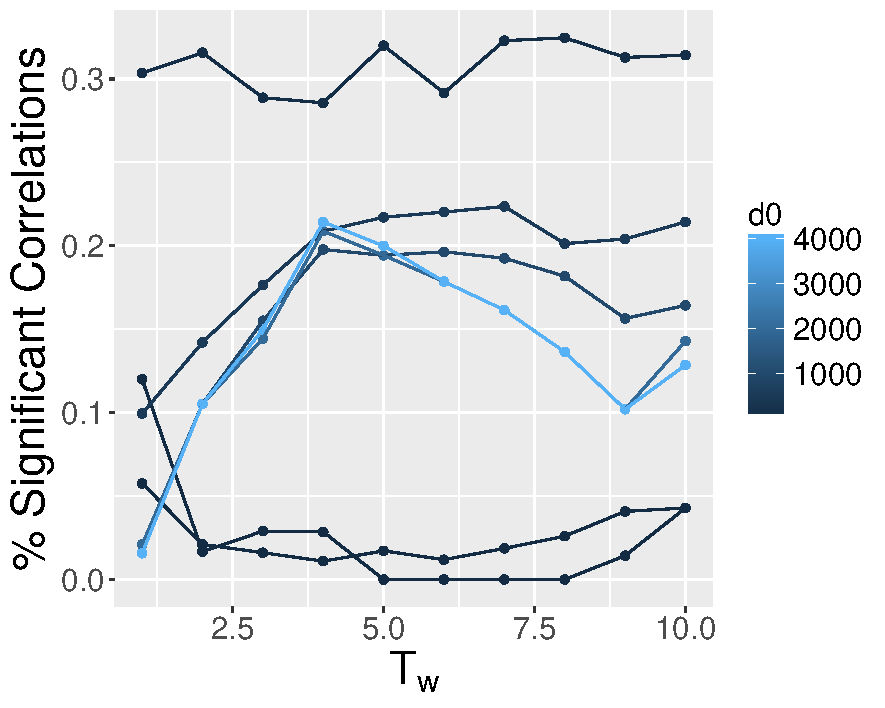
\includegraphics[width=0.48\linewidth]{Figures/MacroCoEvol/significantcorrs_Tw.pdf}
	%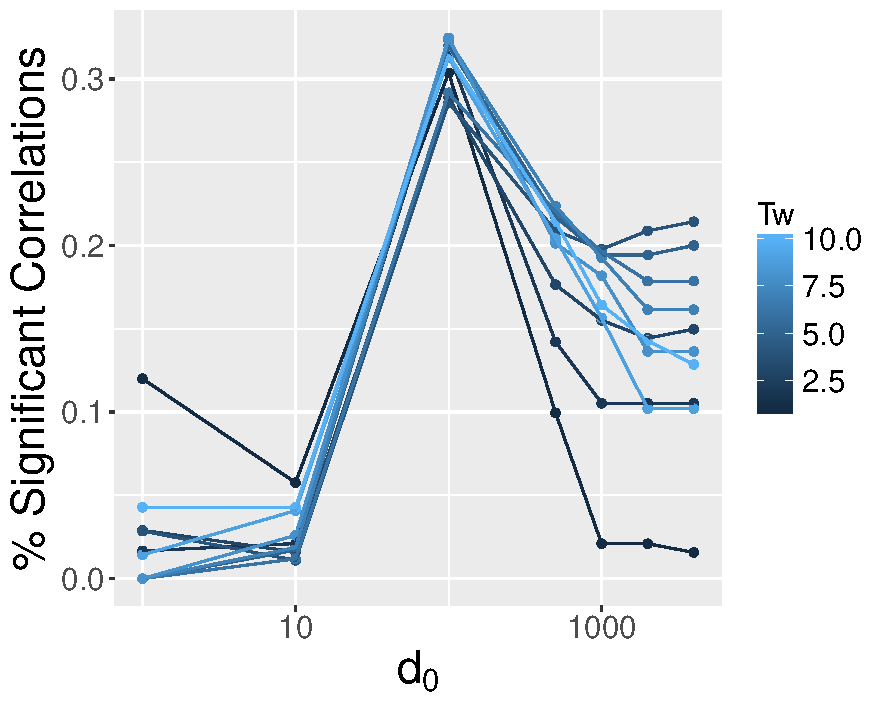
\includegraphics[width=0.48\linewidth]{Figures/MacroCoEvol/significantcorrs_d0.pdf}\\
	%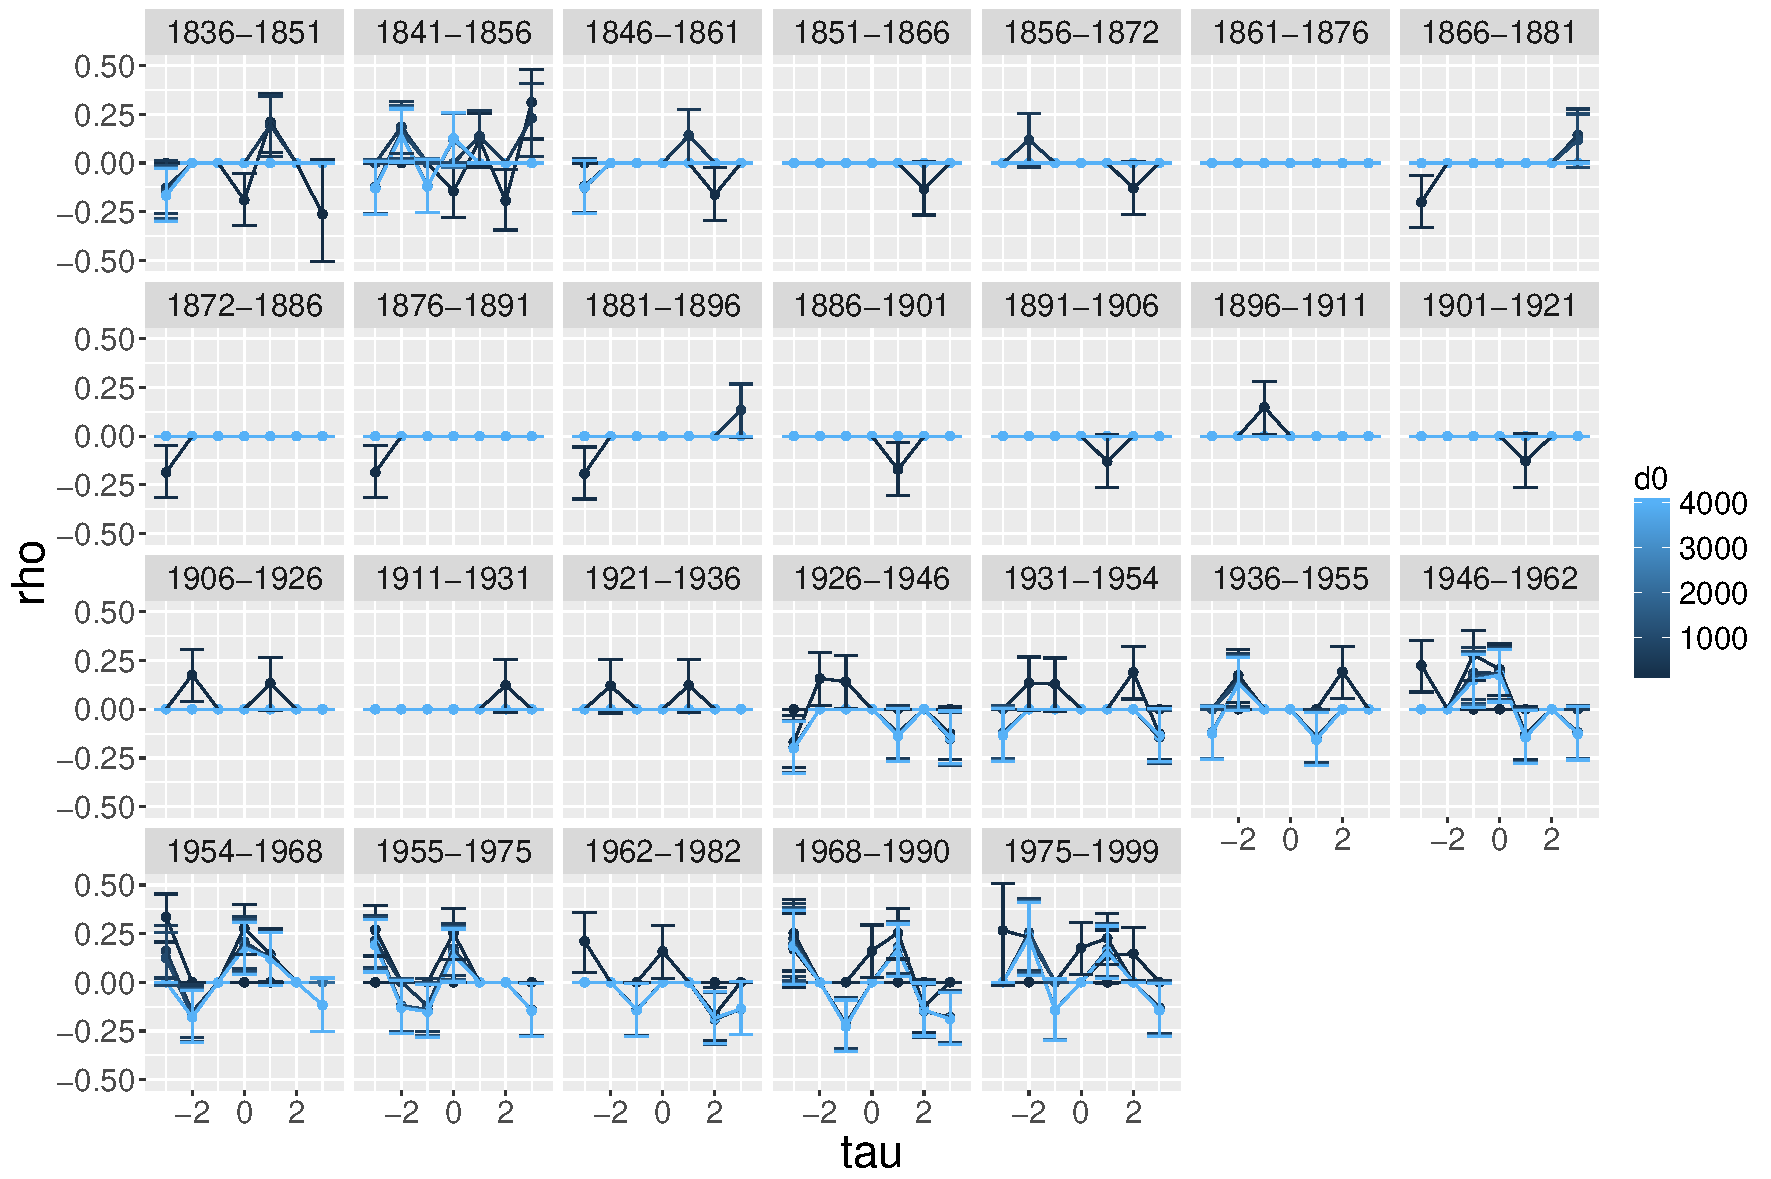
\includegraphics[width=\linewidth]{Figures/MacroCoEvol/laggedCorrs_time_Tw4.pdf}
	\includegraphics[width=\linewidth]{}
	
\end{figure}
%%%%%%%%%%%%%









\subsubsection{Abstract model calibration}{Calibration du modèle abstrait}


\bpar{
Expected results concern both accurate city population growth reproduction, and network patterns, i.e. how does taking into account dynamical networks can introduce further exploratory power in such models for population trajectories, and also how realistic network distance evolution is.
}{
Les résultats attendus de la calibration sur données réelles concernent à la fois la reproduction plus ou moins précise des dynamiques réelles de croissance de population, c'est à dire dans quelle mesure la prise en compte d'un réseau dynamique peut augmenter le pouvoir explicatif pour les trajectoires, et aussi quel est le niveau de réalisme de l'évolution de la distance par le réseau.
}


Questions concrètes à poser au modèle, expériences ciblées : 

\begin{enumerate}
\item le modèle calibre-t-il mieux les populations (en prenant en compte les paramètres supplémentaires)
\item motifs de calibration biobjectif réseau/populations pour le réseau abstrait
\end{enumerate}

\comment[JR]{attention, expliquer le choix des indicateurs de réseau, il faut qu'ils soient adaptés à l'échelle : cf Mimeur nombre d'intersection - relève un peu de la modélisation procédurale.}


\paragraph{Indicators}{Indicateurs}

On peut ajouter aux indicateurs utilisés précédemment un indicateur de calibration pour la distance. L'aspect particulier de l'ajustement pour les populations, qui résidait dans la présence d'une loi de puissance pour les tailles de villes rendant négligeables les performances sur les villes moyennes et les petites villes dans le cas d'une erreur cumulées, et suggérait l'ajout de l'indicateur de l'erreur sur les logarithmes, n'est pas présent pour les distances qui suivent une distribution concentrée sur un ordre de grandeur unique. Nous utilisons ainsi simplement

\[
\varepsilon_D = \log \left[ \sum_t \sum_{i,j} \left(d_{ij}(t) - \tilde{d}_{ij}(t)\right)^2\right]
\]




%%%%%%%%%%%%%
%% ON HOLD : benchmark static model with real network distances


%\paragraph{Role of Real Network Distances}{Rôles des distances réelles de réseau}

%\bpar{
%We use as a benchmark network the geographical shortest paths that have been shown in a previous work to already capture network effects (see~\cite{raimbault2016models} and section~\ref{sec:interactiongibrat}).
%}{
%Nous utilisons comme réseau de benchmark les plus courts chemins géographiques qui ont été montrés déjà capturer des effets de réseaux dans un précédent travail (voir~\cite{raimbault2016models} et la section~\ref{sec:interactiongibrat}).
%}




\paragraph{Results}{Résultats}


Nous procédons à une calibration non-stationnaire, sur les objectifs $(\varepsilon_P,\varepsilon_D)$, par fenêtre mobile sur les périodes deja utilisées en~\ref{sec:interactiongibrat}. Pour limiter la dimension à explorer, nous fixons $w_N = 0$ pour n'étudier les interactions qu'au premier ordre, sachant que les paramètres de réseau abstrait $(g_{max},\gamma_S,\varphi_0)$ sont pris en compte dans la calibration. La Fig.~\label{fig:macrocoevol:pareto} montre les fronts de Pareto obtenus, et la Fig.~\label{fig:macrocoevol:parameters} l'évolution dans le temps des valeurs des paramètres pour les solution optimales.


%%%%%%%%%%%%%%%%%%%
\begin{figure}
	%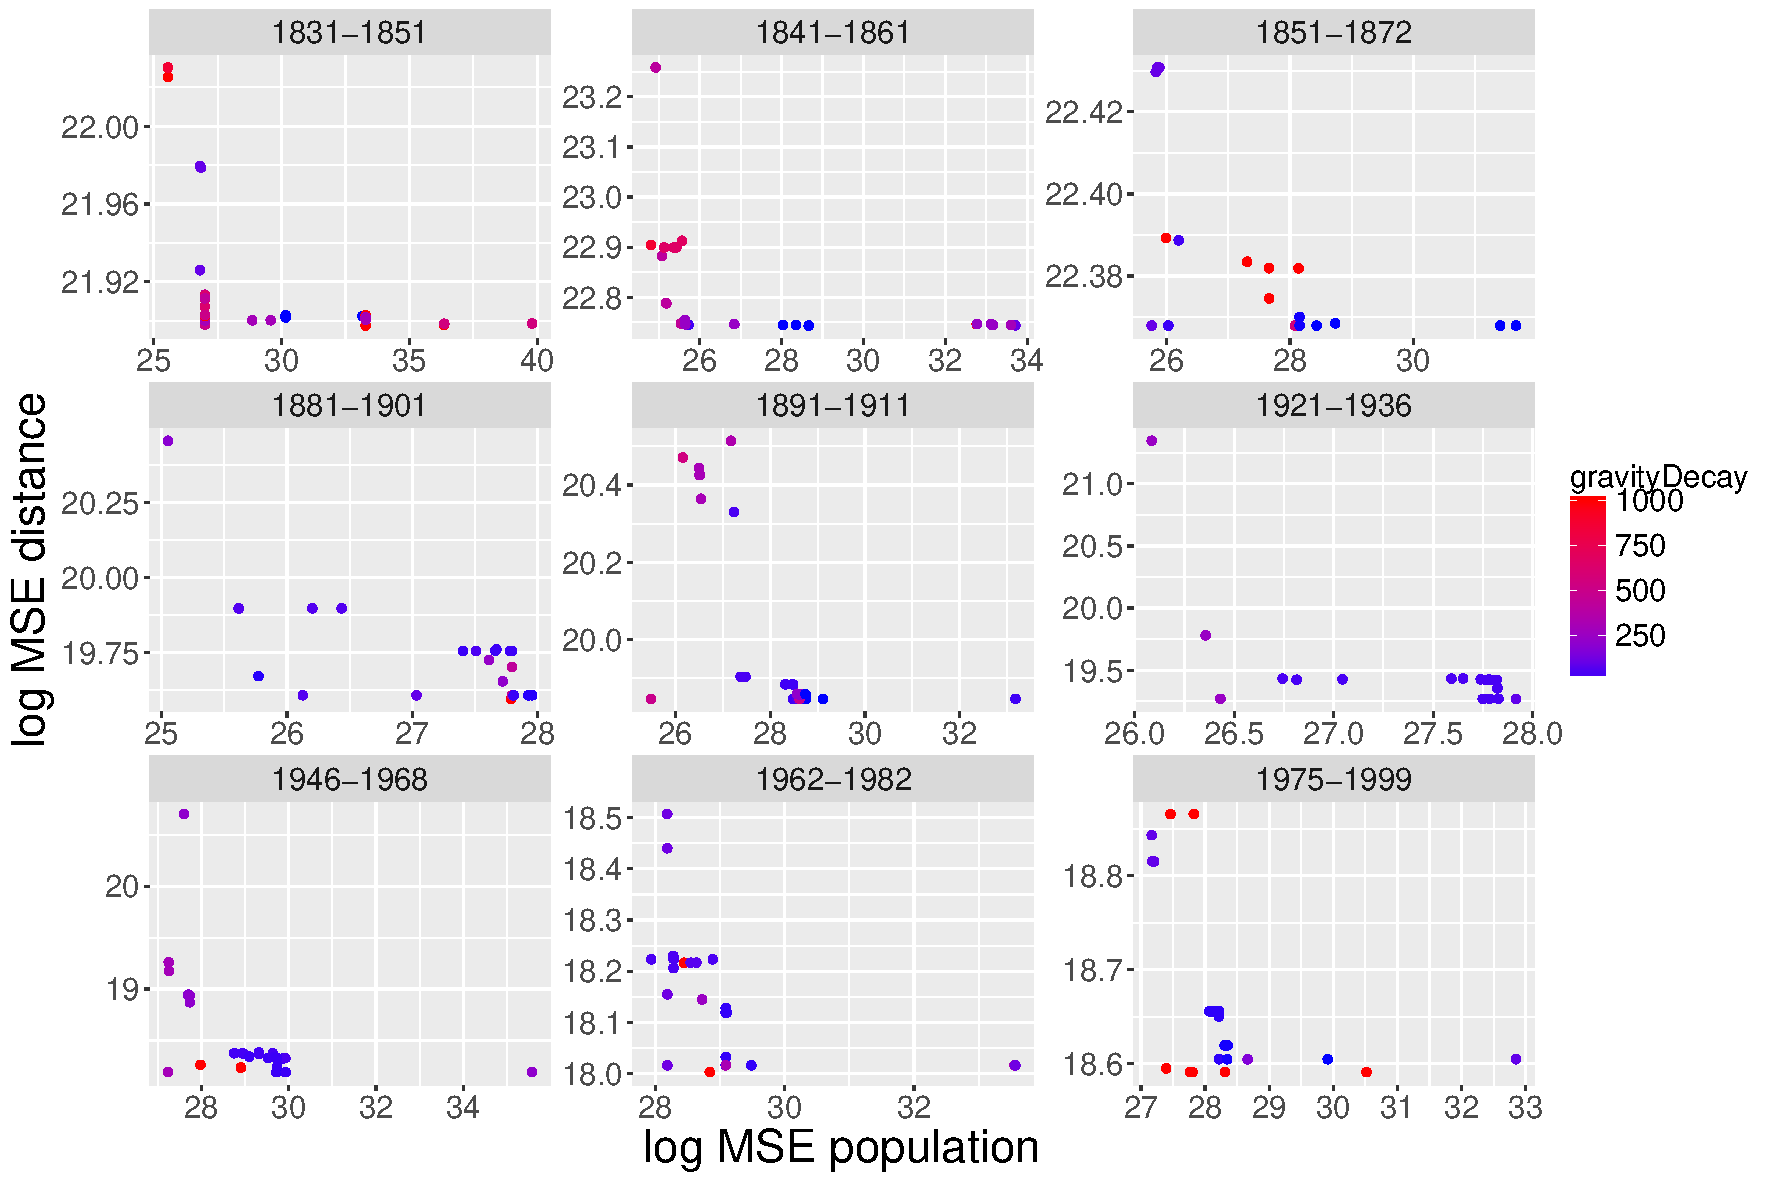
\includegraphics[width=0.9\linewidth]{Figures/MacroCoEvol/pareto_gravityDecay}\\
	%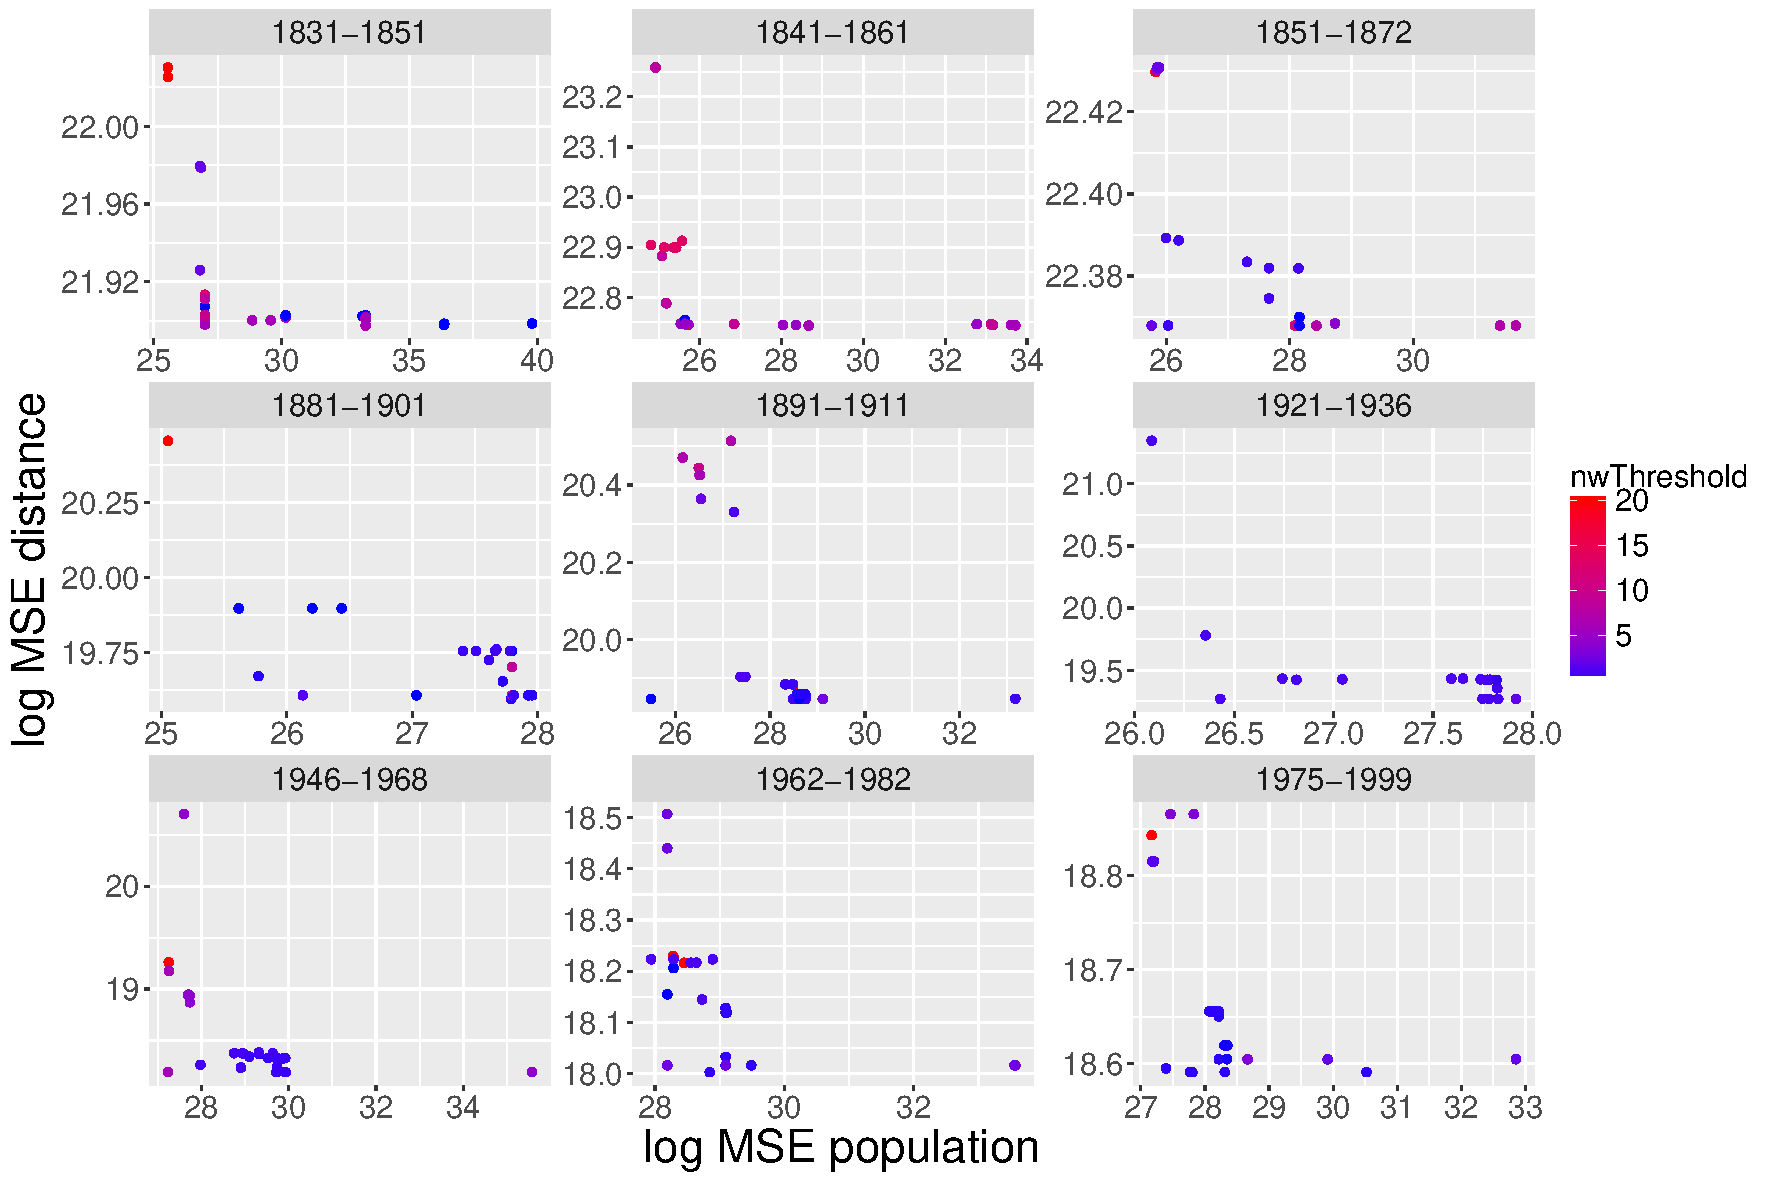
\includegraphics[width=0.9\linewidth]{Figures/MacroCoEvol/pareto_nwThreshold}
	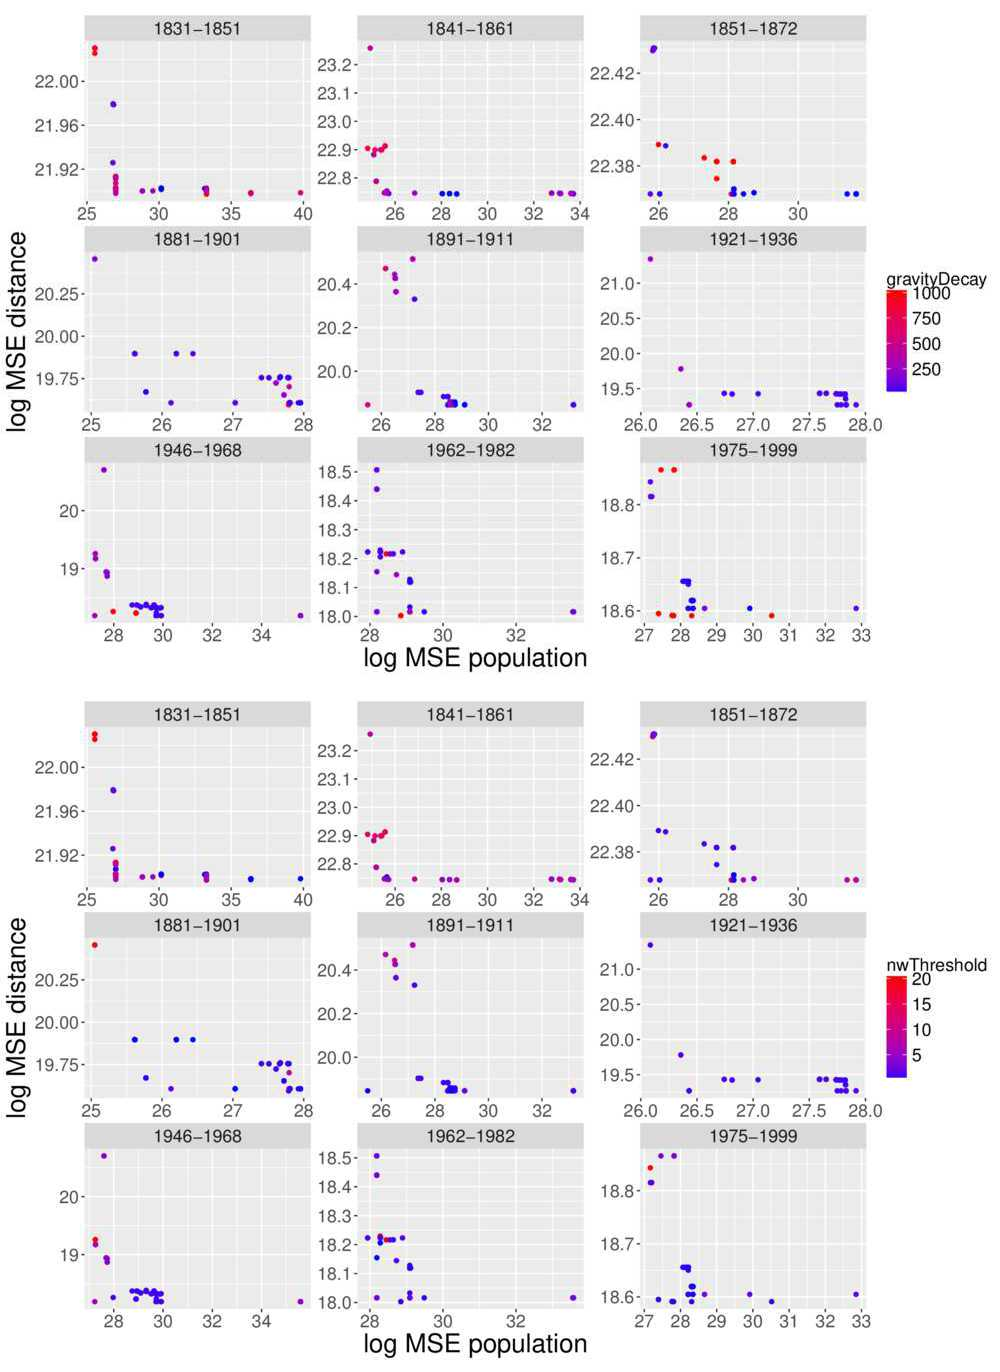
\includegraphics[width=\linewidth]{Figures/Final/6-2-3-fig-macrocoevol-pareto}
	\caption[Pareto fronts][Fronts de Pareto]{\label{fig:macrocoevol:pareto}}{\textbf{Fronts de Pareto pour la calibration bi-objectif population et distance.}\label{fig:macrocoevol:pareto}}
\end{figure}
%%%%%%%%%%%%%%%%%%%


%%%%%%%%%%%%%%%%%%%
\begin{figure}
	%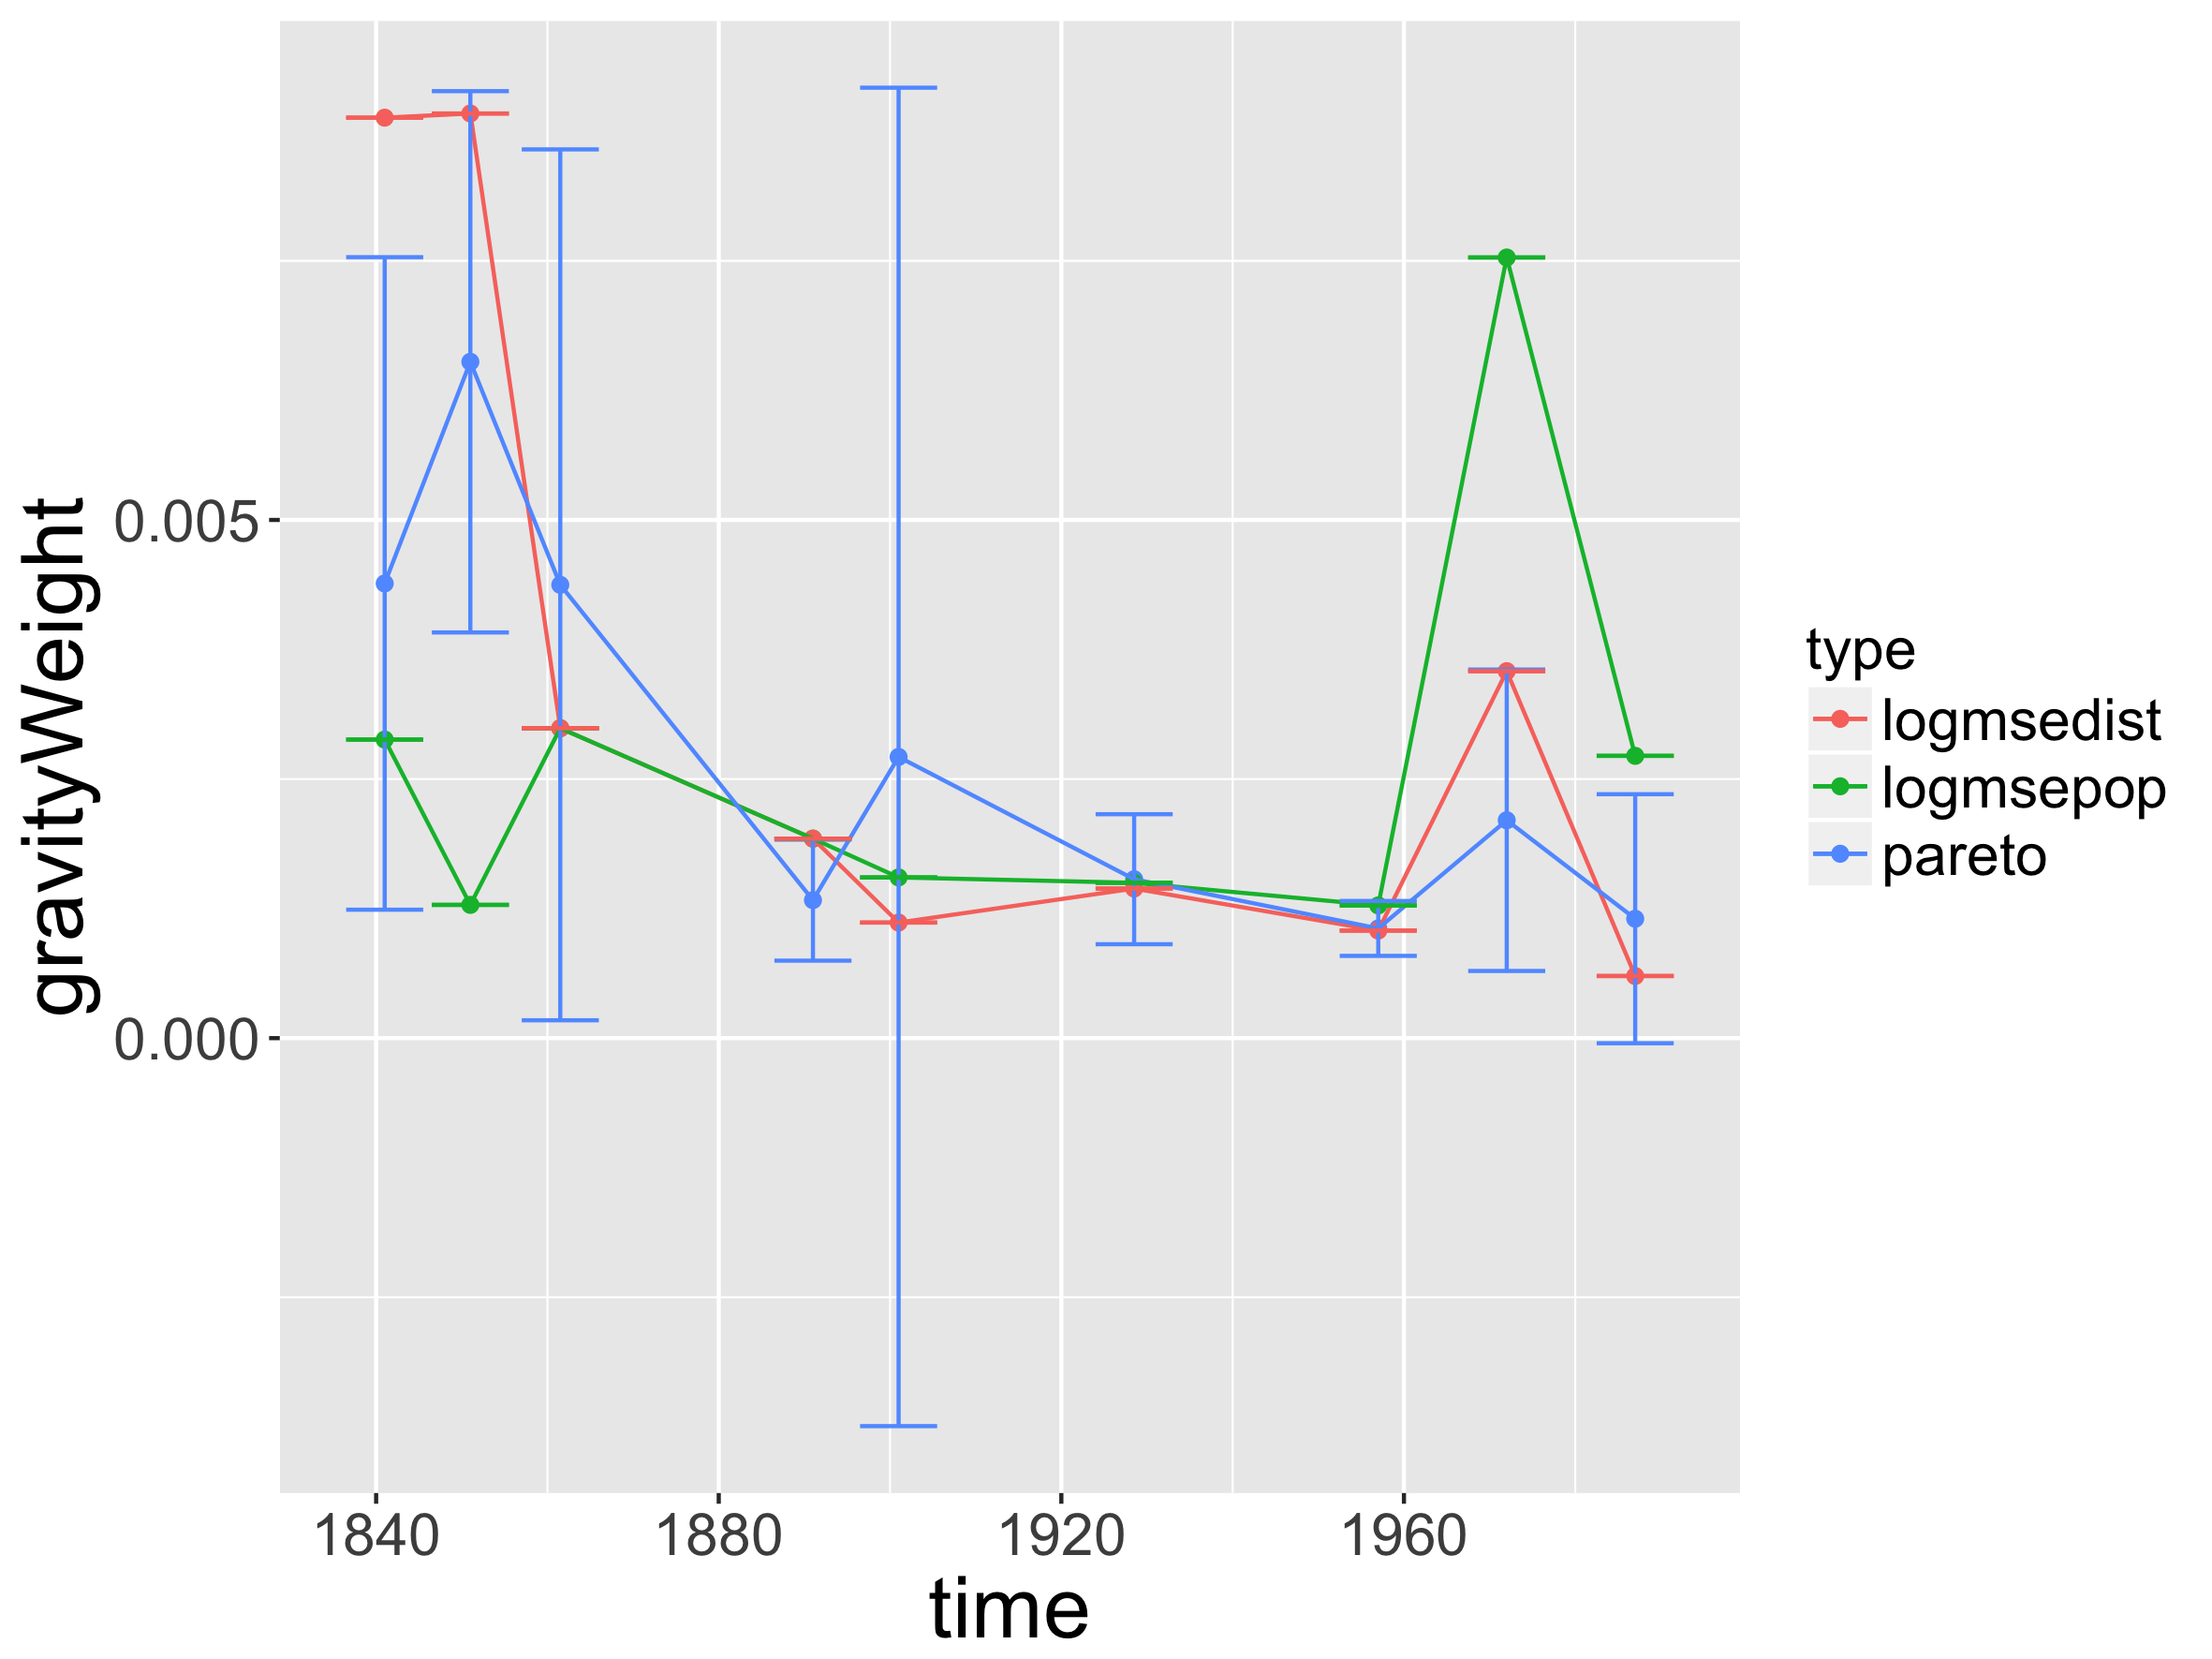
\includegraphics[width=0.32\linewidth]{Figures/MacroCoEvol/param_gravityWeight_filt1}
	%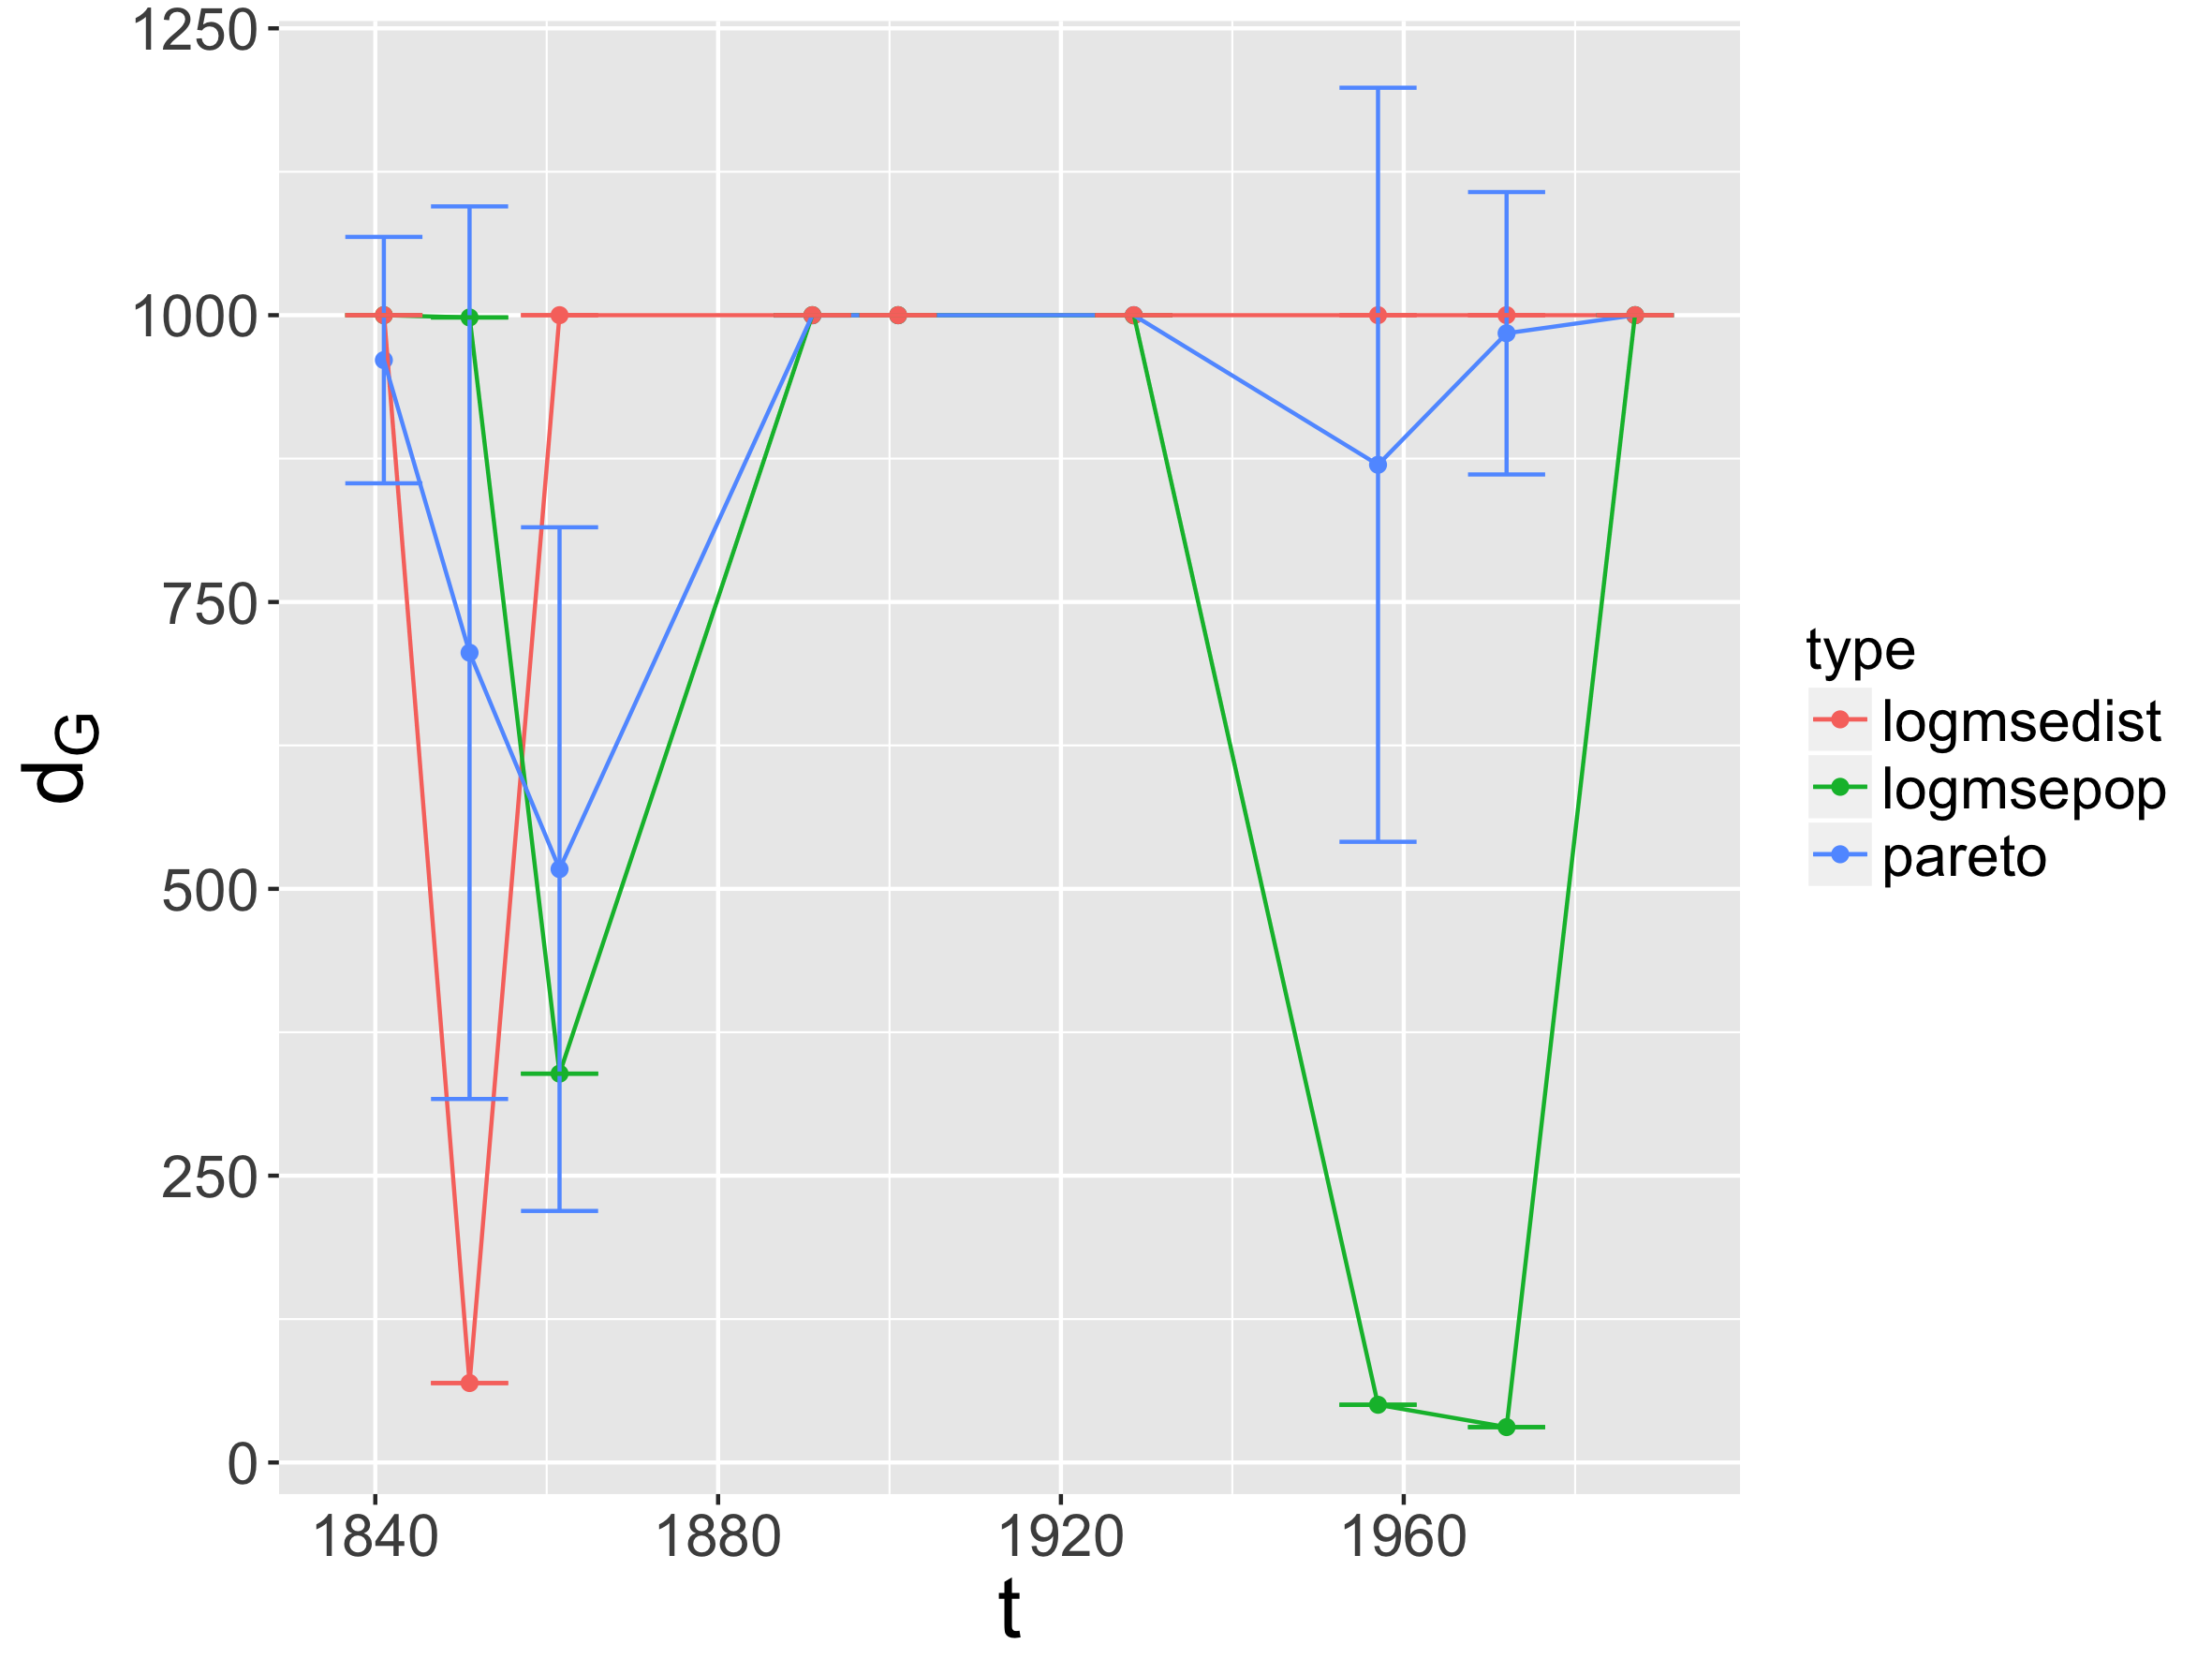
\includegraphics[width=0.32\linewidth]{Figures/MacroCoEvol/param_gravityDecay_filt1}
	%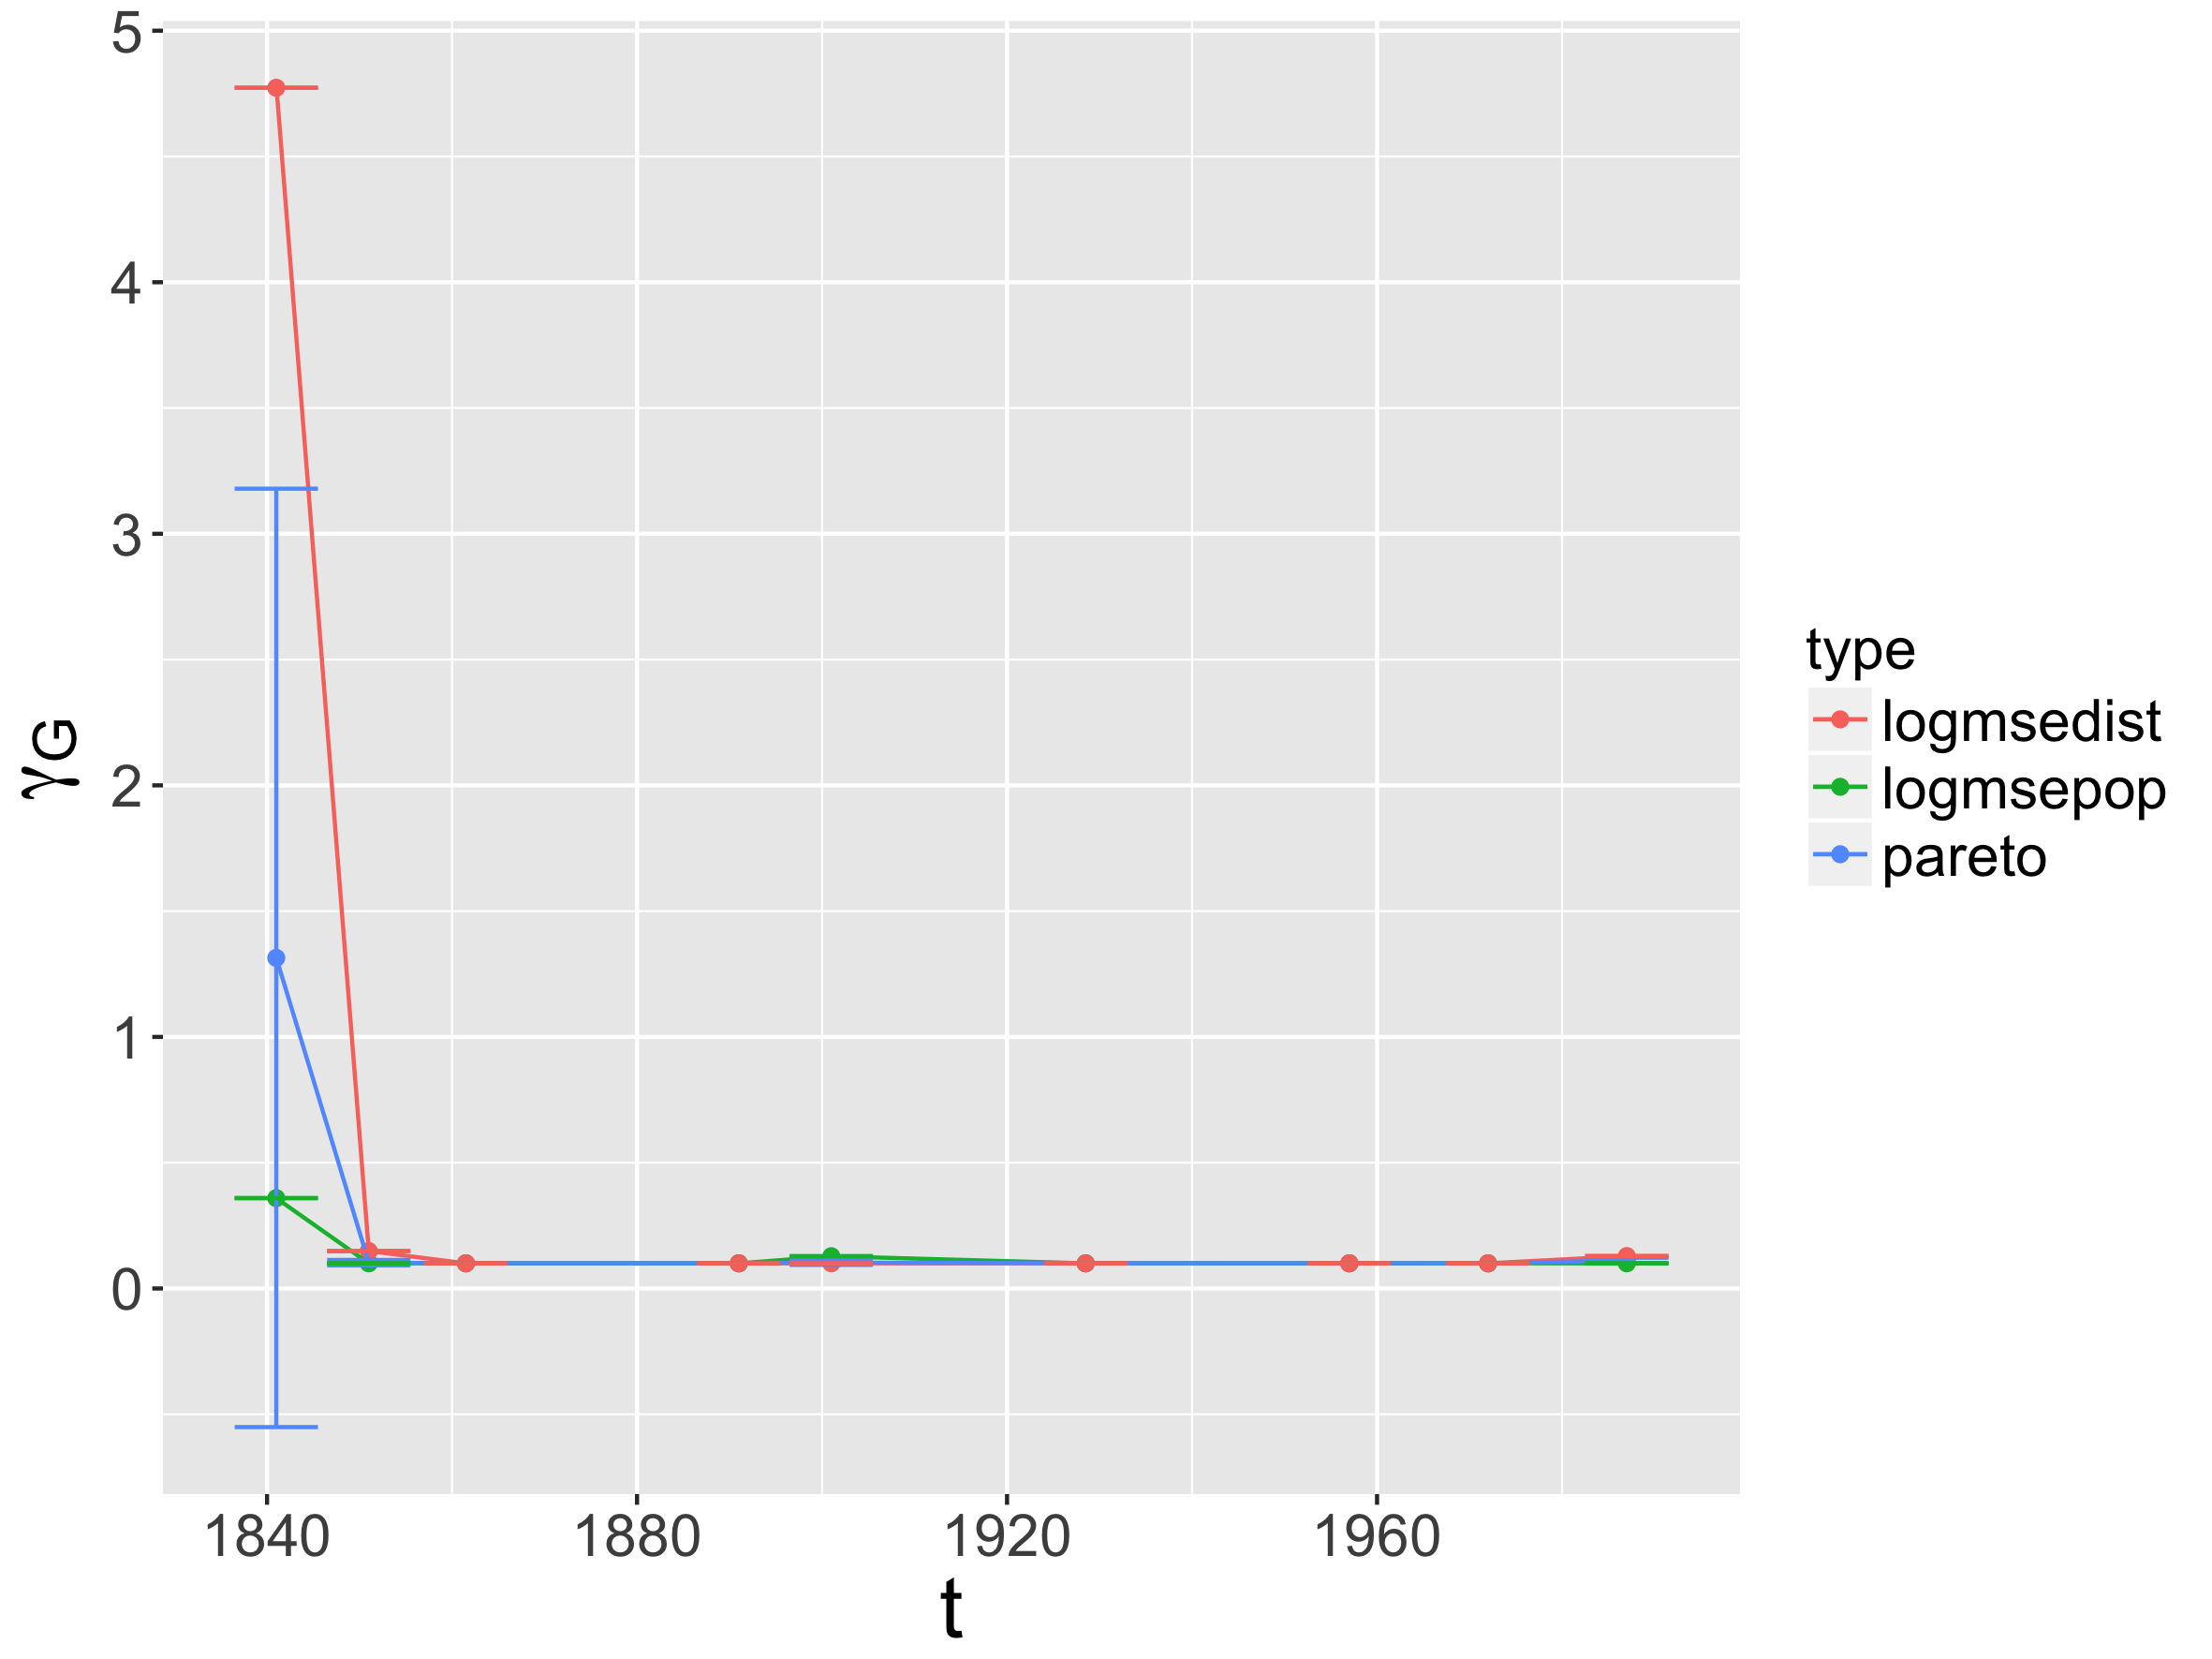
\includegraphics[width=0.32\linewidth]{Figures/MacroCoEvol/param_gravityGamma_filt1}\\
	%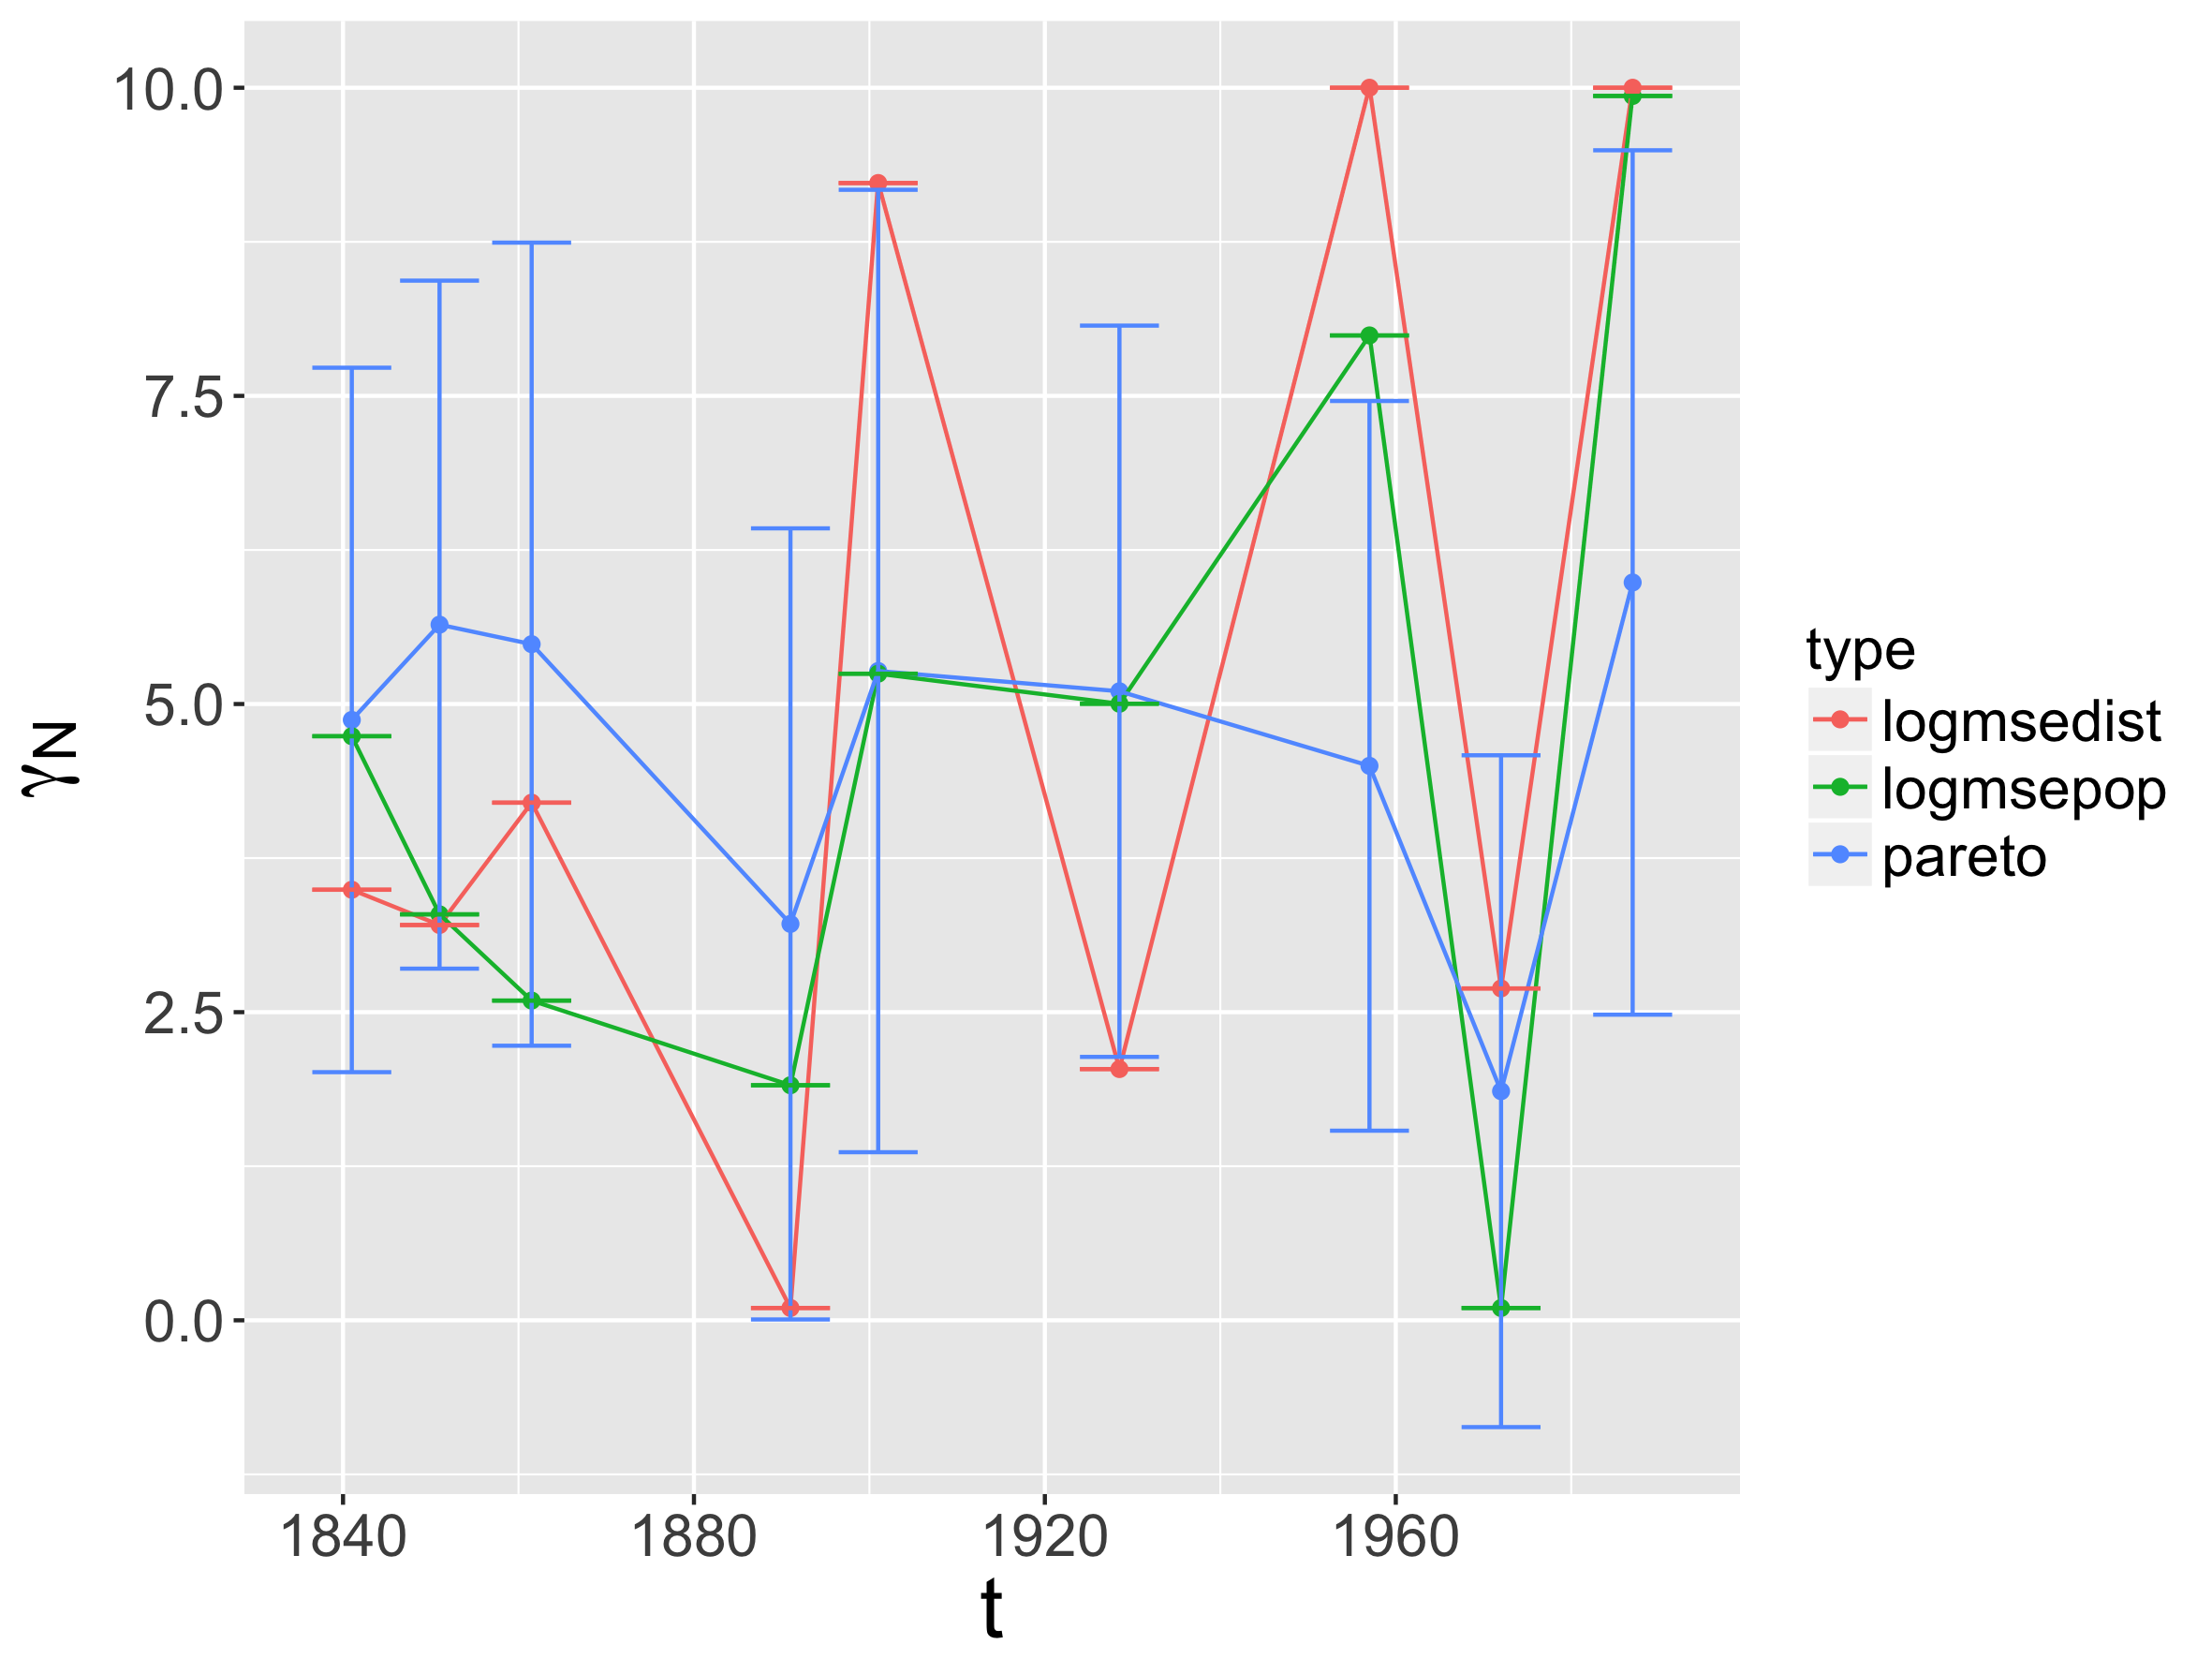
\includegraphics[width=0.32\linewidth]{Figures/MacroCoEvol/param_nwExponent_filt1}
	%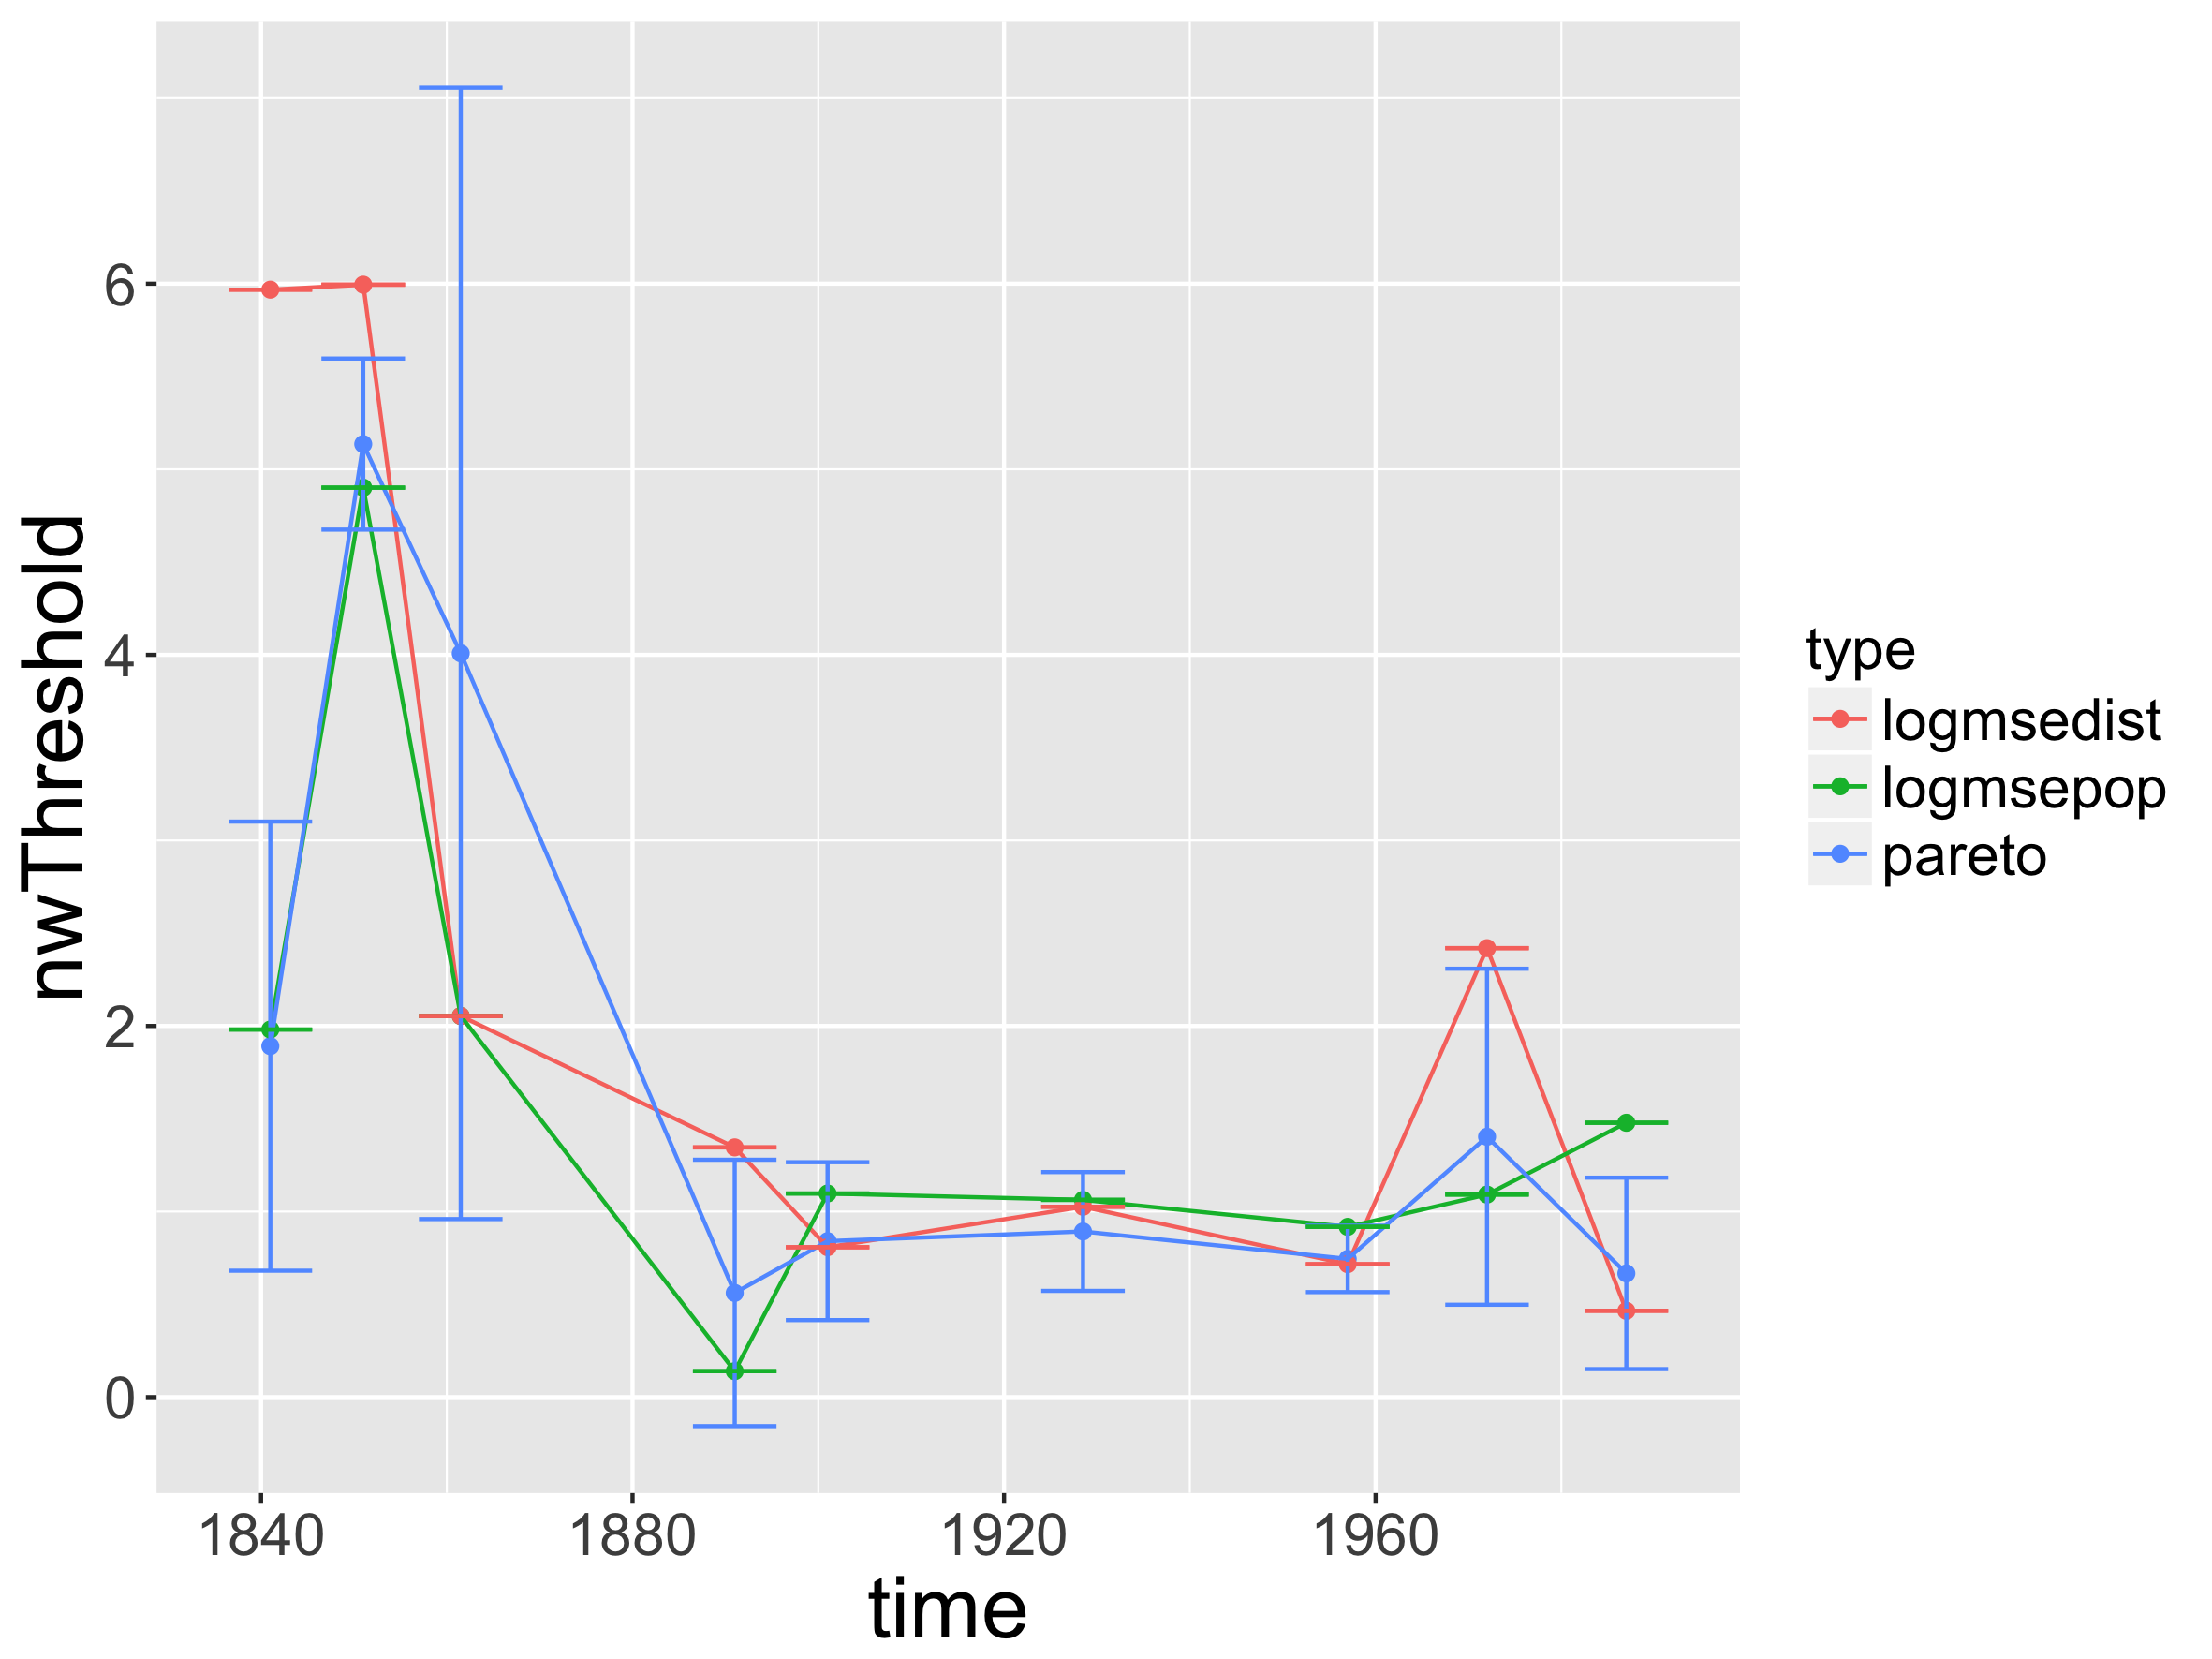
\includegraphics[width=0.32\linewidth]{Figures/MacroCoEvol/param_nwThreshold_filt1}
	%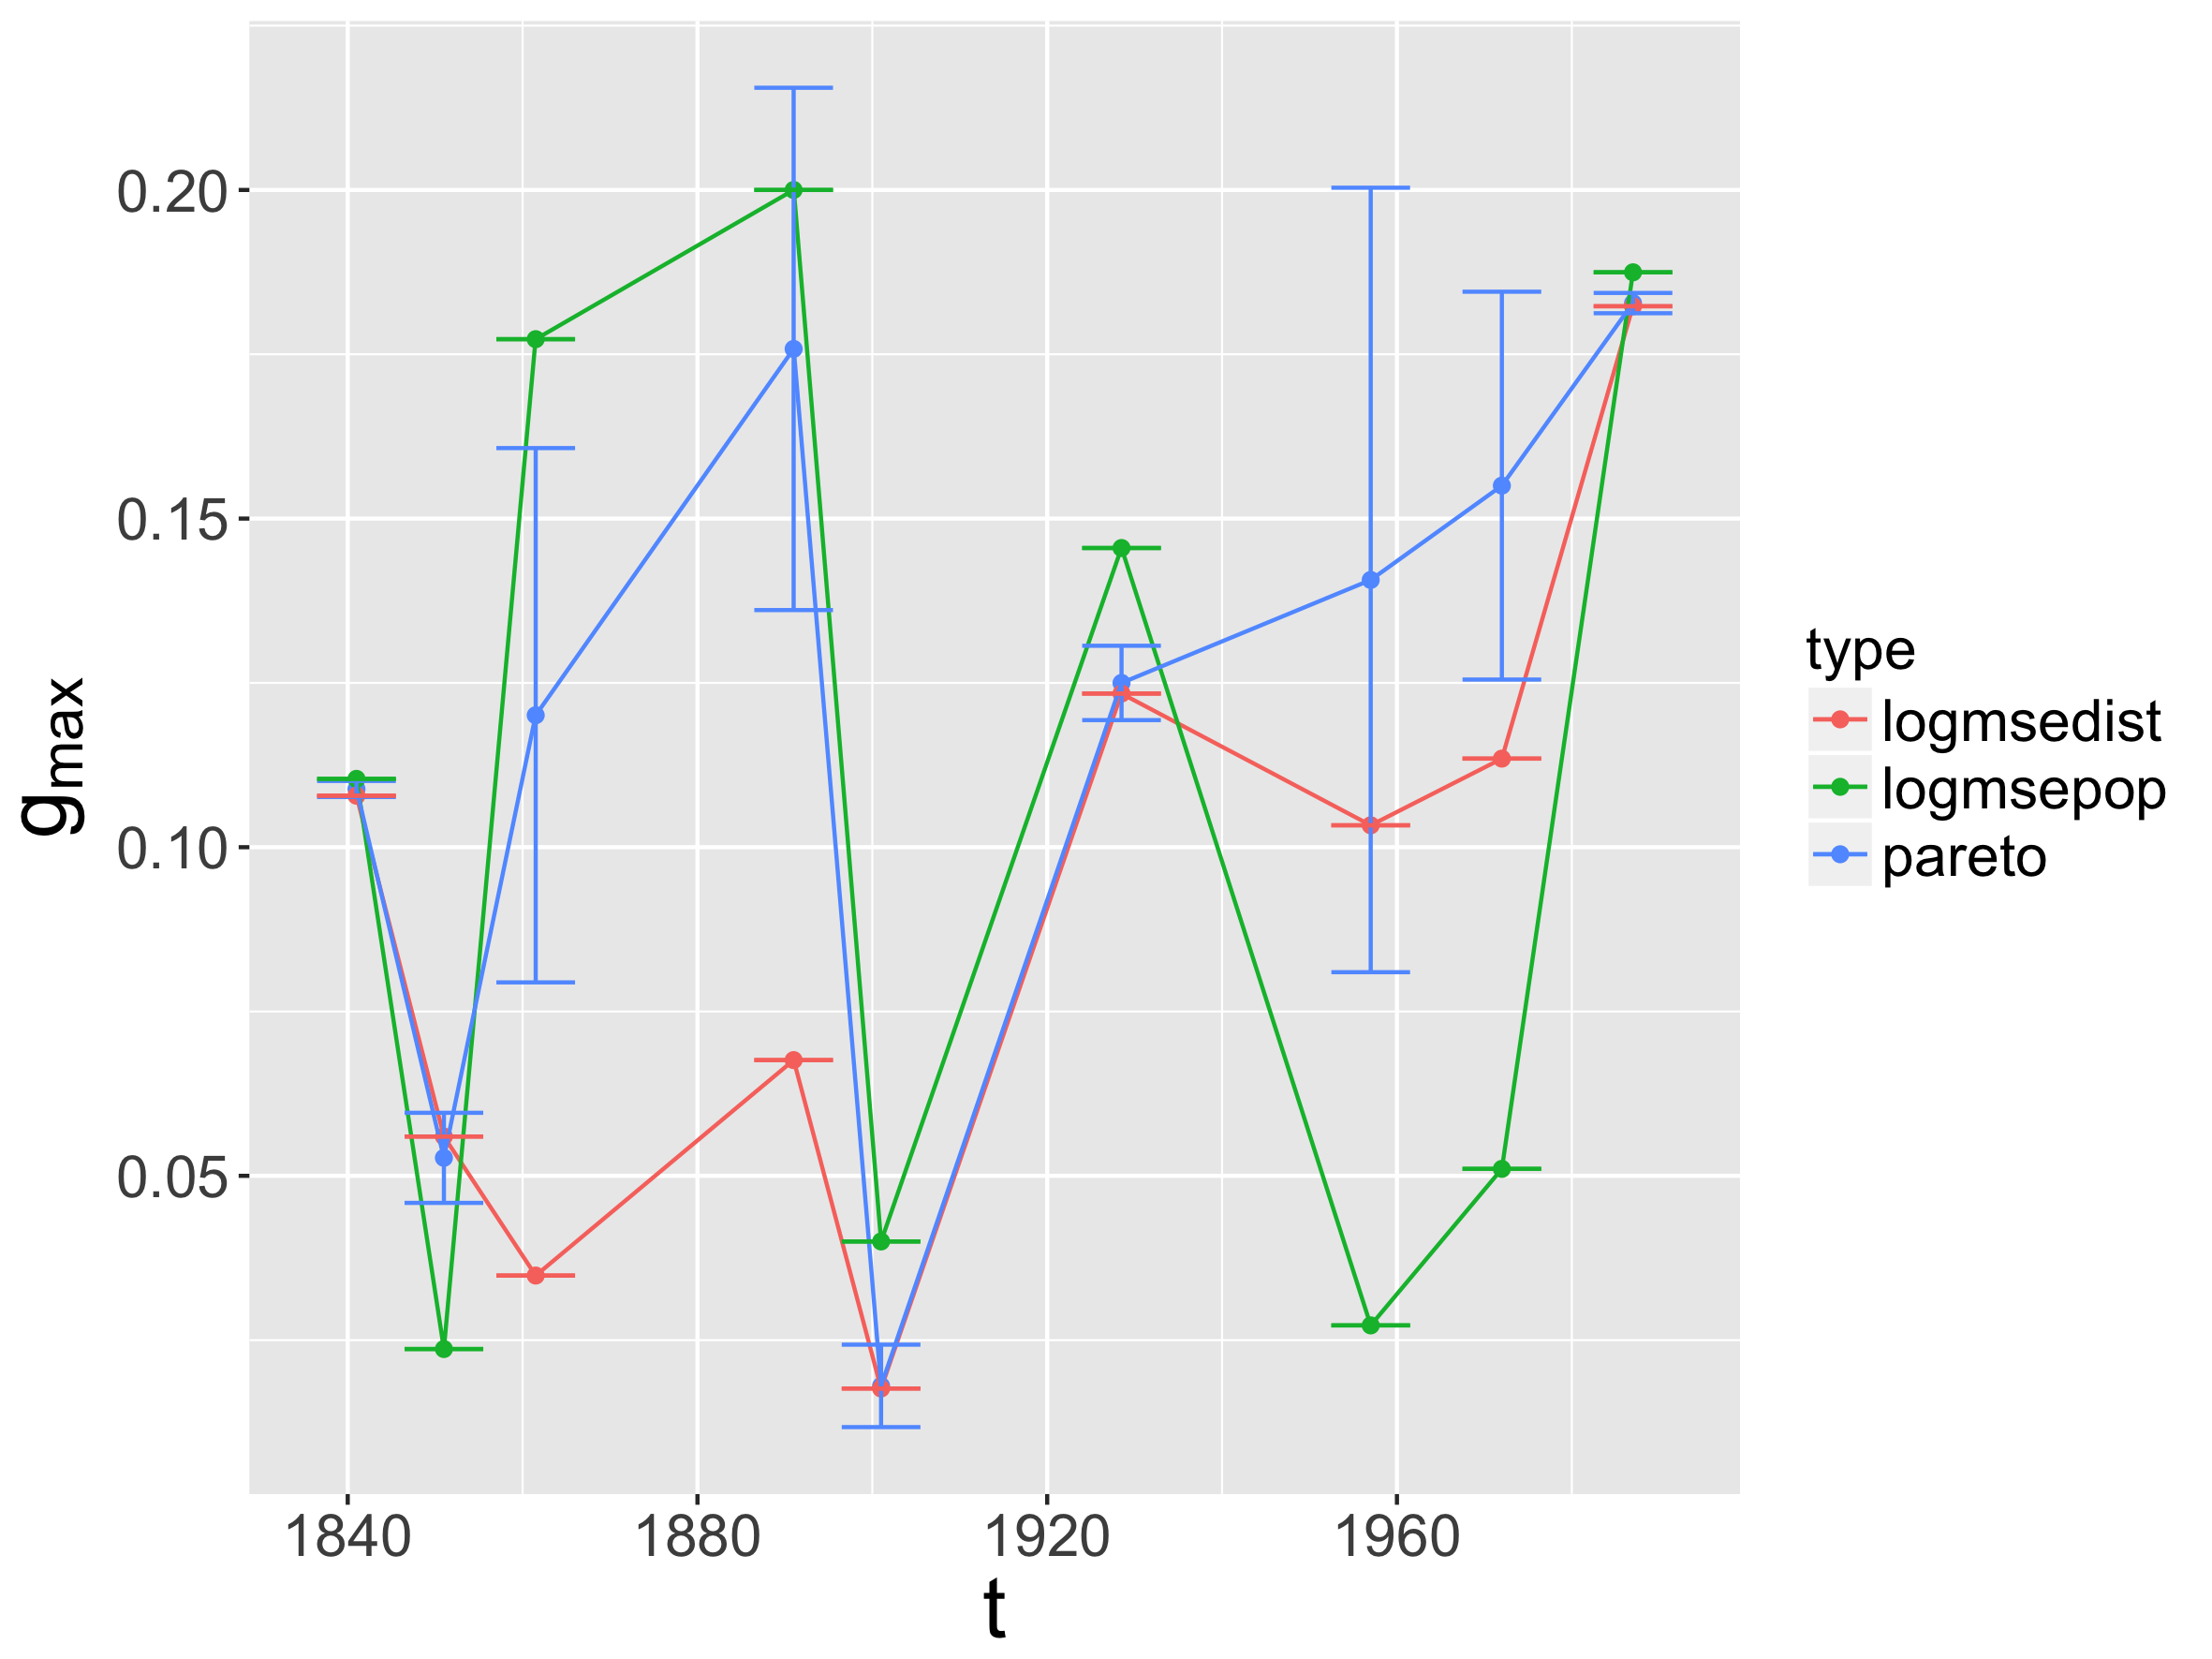
\includegraphics[width=0.32\linewidth]{Figures/MacroCoEvol/param_nwGmax_filt1}
	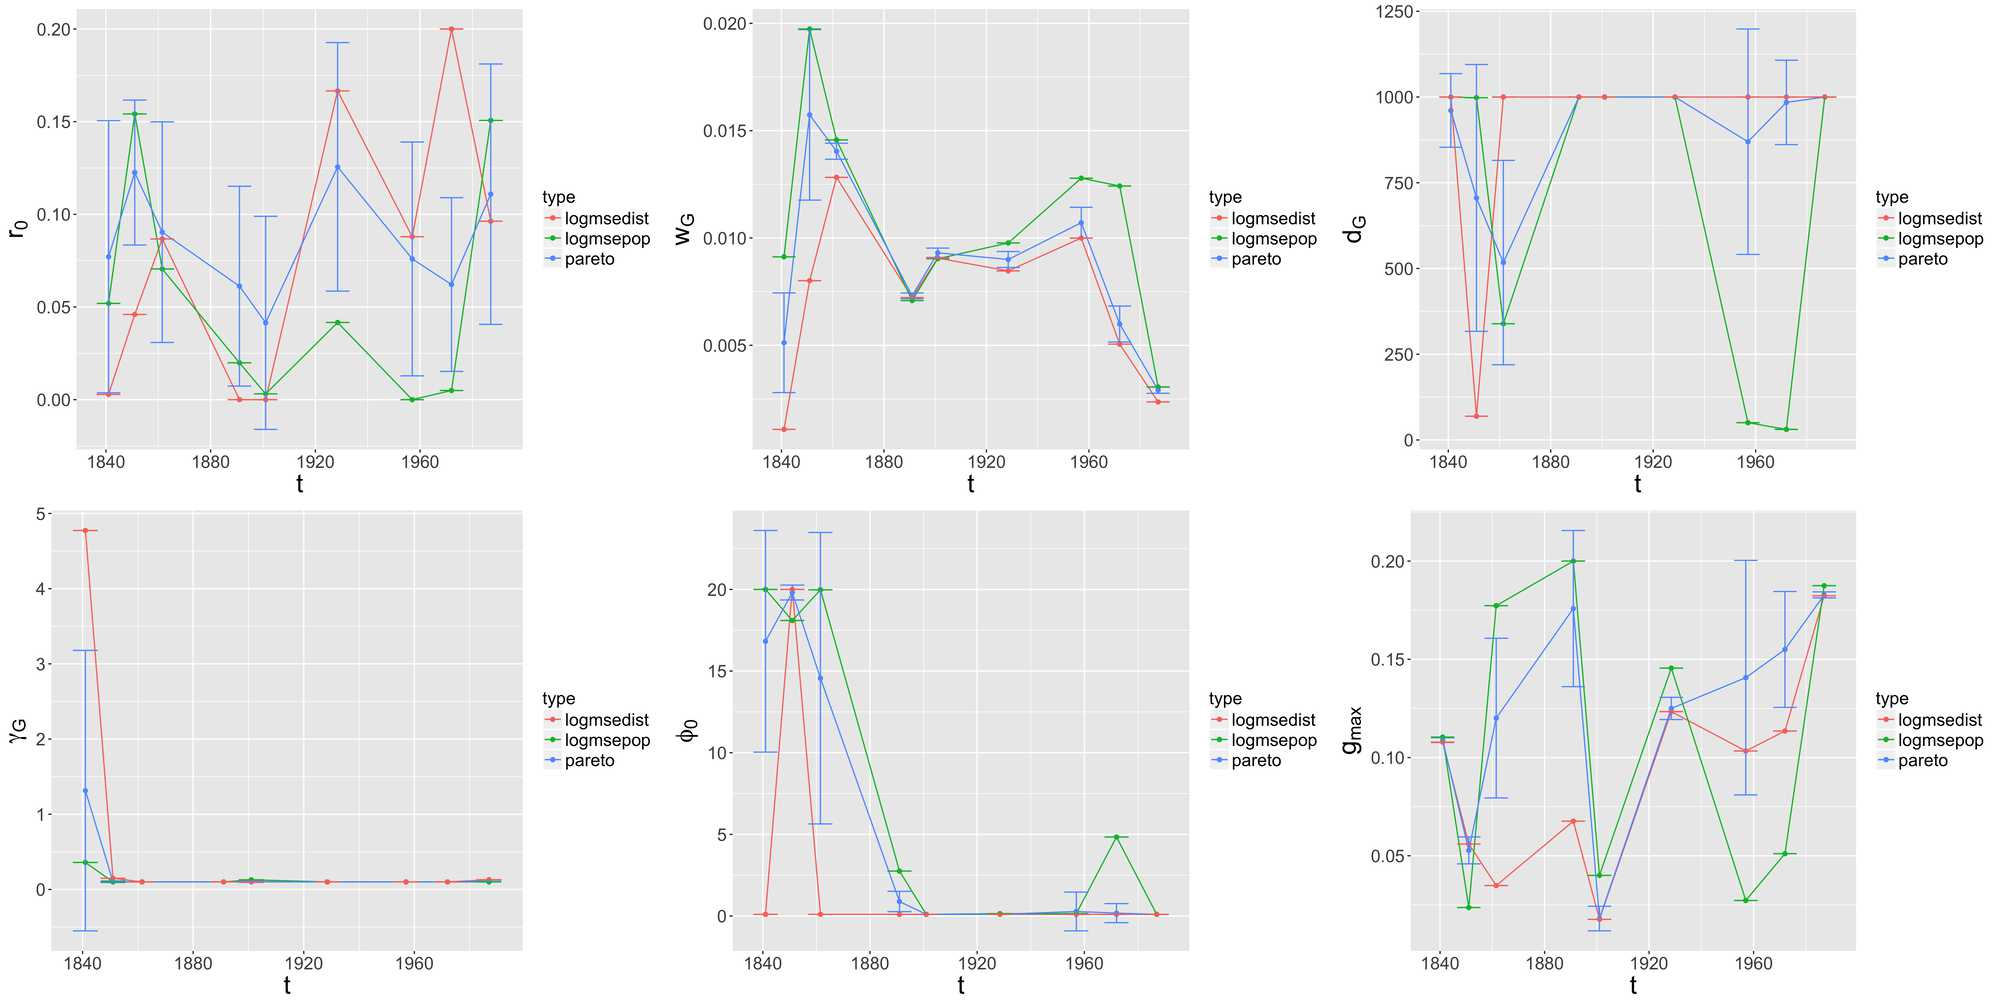
\includegraphics[width=\linewidth]{Figures/Final/6-2-3-fig-macrocoevol-parameters.jpg}
	\caption[][Evolution des paramètres optimaux]{\label{fig:macrocoevol:parameters}}{\textbf{Evolution temporelle des paramètres optimaux.}\label{fig:macrocoevol:parameters}}
\end{figure}
%%%%%%%%%%%%%%%%%%%








\subsubsection{Physical network}{Modèle avec réseau physique}


% exemple avec slime-mould

Q : reciprocally how can such coupled models produce realistic networks compared to more classical autonomous models of network growth.

La spécification avec réseau physique correspond en un sens à la combinaison de différentes échelles



Dans le cas d'un auto-renforcement, une specification similaire à celle utilisée précédemment suppose une croissance pour l'ensemble des liens :

\[
d(t+1) = d(t)\cdot \left(1 + g_{max} \cdot \left[\frac{\phi}{\max \phi}\right]^{\gamma_s}\right)
\]

la specification par seuil ne permettant pas une bonne convergence dans le temps.

Un exemple de configuration obtenue par cette spécification est donné en Fig.~\ref{fig:macrocoevolution:slimemould}.


%%%%%%%%%%%%%%%%%%%%%%
\begin{figure}
	%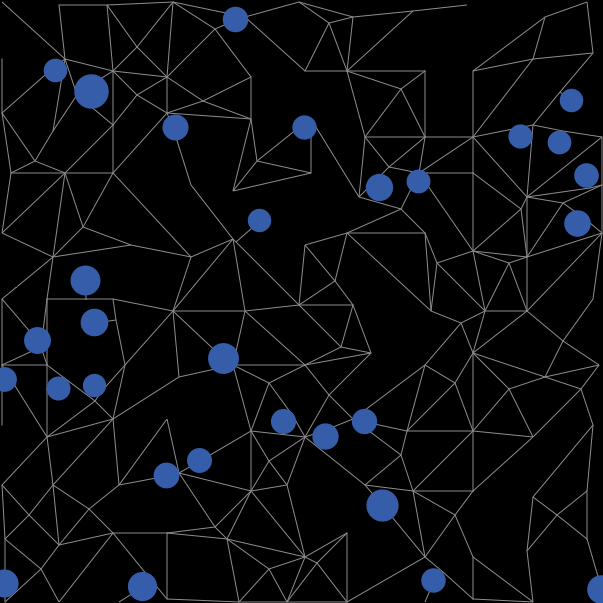
\includegraphics[width=0.45\linewidth]{Figures/MacroCoEvol/example_slimemould_1_t0}
	%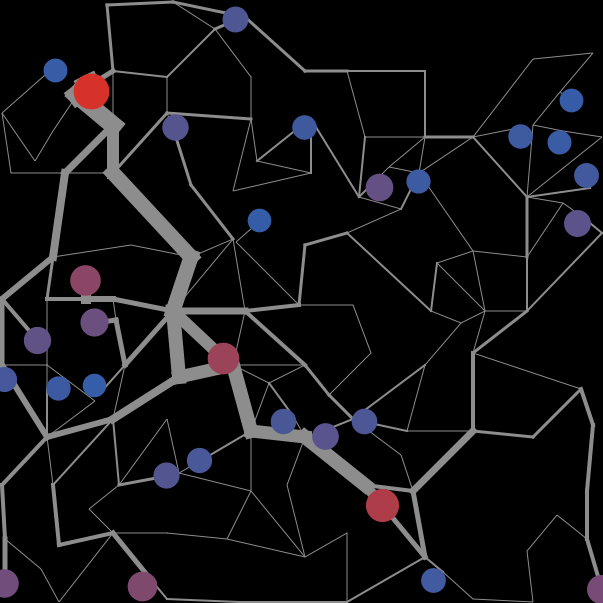
\includegraphics[width=0.45\linewidth]{Figures/MacroCoEvol/example_slimemould_1_tf}
	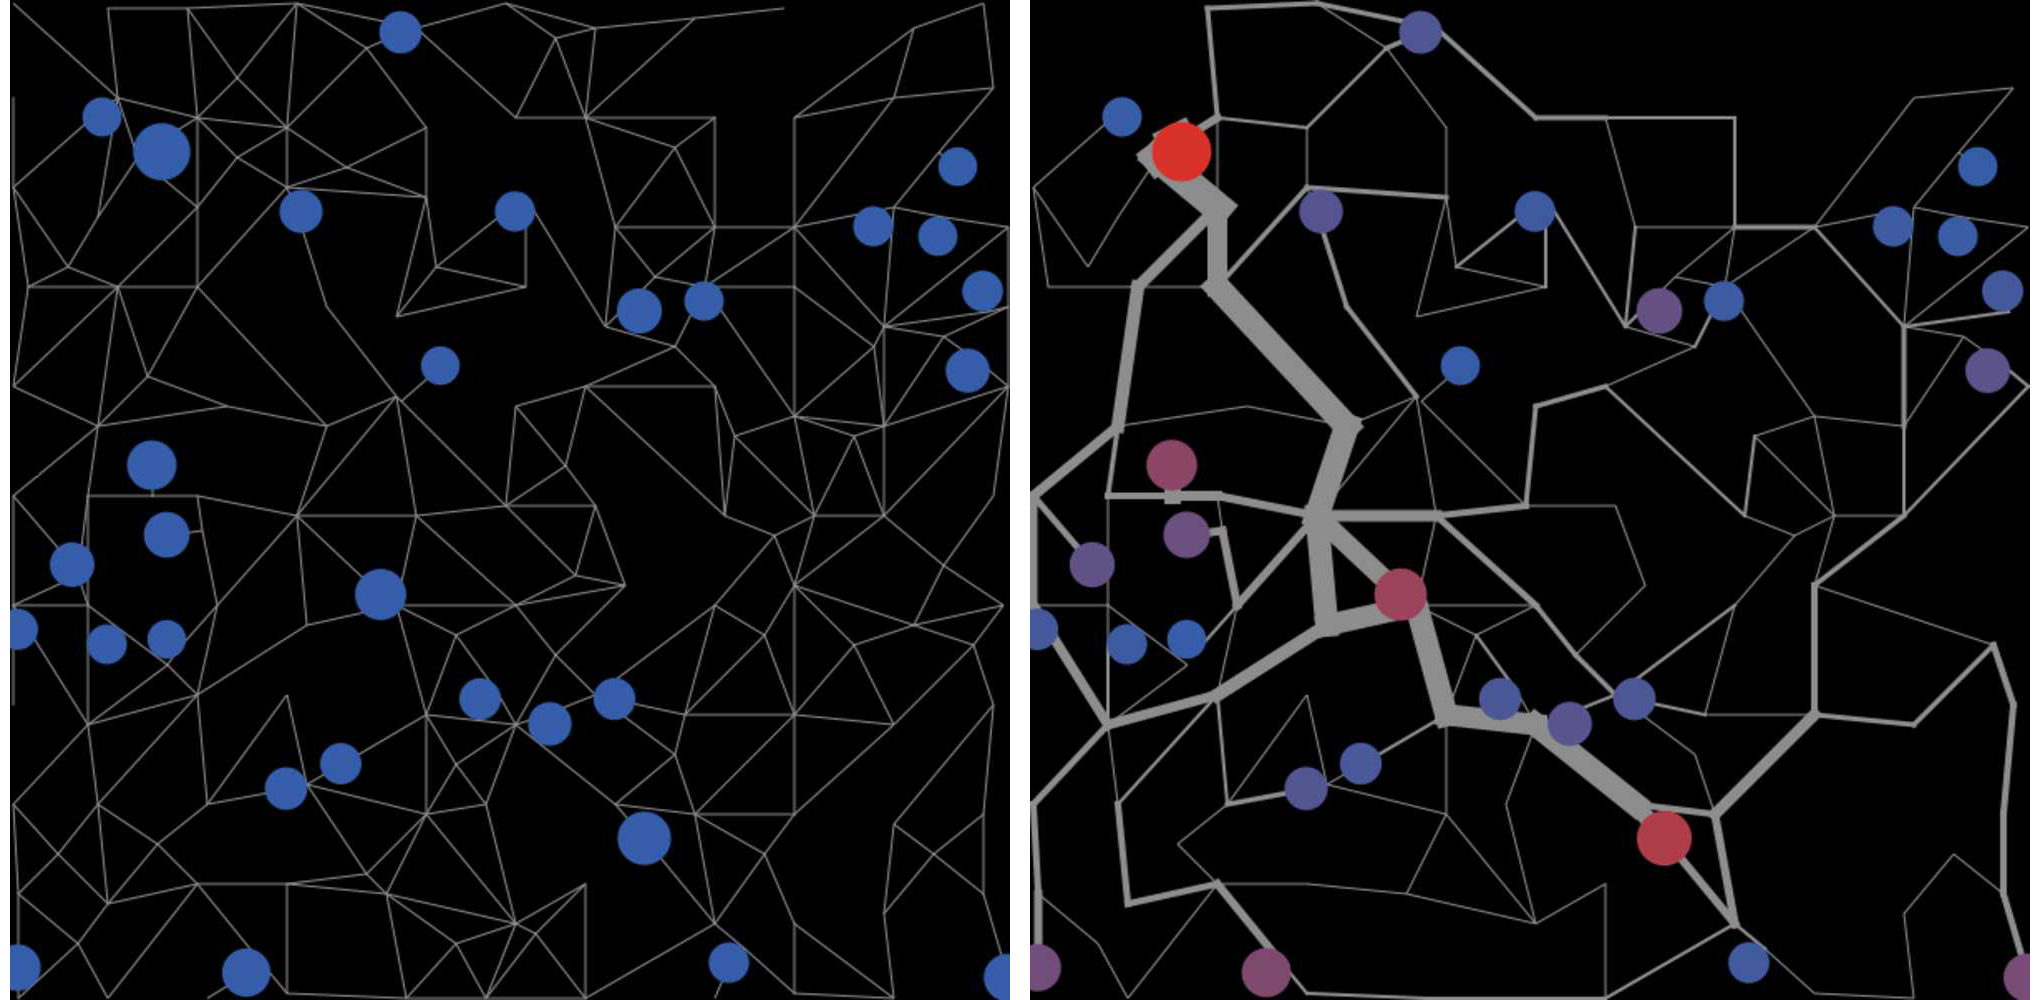
\includegraphics[width=\linewidth]{Figures/Final/6-2-3-fig-macrocoevol-slimemould}
	\caption[][Example de réseau auto-renforçant]{}{\textbf{Example de configuration obtenue avec réseau auto-renforçant.} \textit{(Gauche)} Configuration initiale aléatoire, capacités égales ; \textit{(Droite)} Configuration finale obtenue après 100 itérations.\label{fig:macrocoevolution:slimemould}}
\end{figure}
%%%%%%%%%%%%%%%%%%%%%%


%%%%%%%%%%%%%%%%%
%% ON HOLD


%\begin{enumerate}
%\item le modèle produit-il des formes de réseau crédibles dans le cas du réseau physique ?
%\item éventuellement si les correlations temporelles sont calculées sur les vrais données, le modèle peut-il être calibré au second ordre (sur les correlations/causalités) ?
%\end{enumerate}


%\comment{\cite{mimeur:tel-01451164} la thèse de Mimeur est un pont intéressant entre géographie et approches éco de Levinson (modèle de croissance type slime mould ?). plus fait des stats spatiales pour lier croissance pop et accessibilité : checker si même résulats quand fera spatio-temp causalities sur réseau ferré et autoroutier et croissance pop. remarque : trucs bizzares, essaie d'expliquer pour petites villes, mais pas approprié, pb du choix de l'échelle, de ce qui est du bruit et du signal - semble tout mélanger : importance du preprocessing et traitement du signal (cf correlations des taux de croissance). Tester effets fixes régions/départements ? fait GWR finalement ?}




\subsubsection{Possible Developments}{Développements possibles}

\paragraph{Multi-layer network}{Réseau multi-couches}

\bpar{
Specifically-designed database of the highway networks containing its full genesis from 1950 to 2015).
}{
La considération d'un seul mode de transport pour le système réel est bien sûr réductrice, et une direction immediate de développement est d'une part le test du modele avec des matrices de distance réelles pour d'autres types de réseaux, comme le réseau autoroutier qui a connu un essor considerable en France entre 1950 et 1999. Cette application nécessite la mise en place d'une base dynamique pour la croissance du réseau couvrant 1950 à 2015, les bases classiques (IGN ou OpenStreetMap n'integrant pas la date d'ouverture des tronçons). Une extension naturelle du modele consisterait alors en la mise en place d'un réseau multi-couches, approche typique pour représenter des systèmes de transport multi-modaux~\cite{gallotti2014anatomy}. Chaque couche du réseau de transport devrait avoir une dynamique co-evolutive avec les populations, avec possiblement l'existence d'une dynamique inter-couches.
}


\paragraph{Particular trajectories}{Trajectoires Particulières}


\bpar{
The role of medium-sized cities on the trajectories of the system can also be examined with the model.
}{
L'étude de trajectoires particulières au sein du système de villes peut permettre de répondre à des questions thématiques spécifiques : par exemple, l'influence des villes moyennes sur la trajectoire globale du système, ou les déterminants d'une plus ou moins bonne ``réussite'' pour ce type de profil.
}




\paragraph{Comparison of Urban Systems}{Comparaison de systèmes urbains}


\bpar{
Finally, a comparison between the urban systems in different geographical and political contexts and at different scales should unveil implications of planning on the interactions between networks and cities, for example by comparing the rather bottom-up growth of the French railway network to the top-down state-planned French highway and Chinese HSR networks.
}{
On s'attend finalement également à pouvoir par l'intermédiaire de ce modele comparer des systèmes urbains dans des contextes géographiques et politiques différents, ainsi qu'a différentes échelles. Cela devrait permettre de révéler les implications des actions de planification sur les interactions entre réseaux et territoires. Par exemple, le réseau ferre français a emerge de manière relativement auto-organisée (de par les multiples opérateurs), tandis que les autoroutes ont été fortement planifiées, a l'image du réseau ferré à grande vitesse Chinois, pour lequel un développement précis est envisagé.
}









